% Options for packages loaded elsewhere
\PassOptionsToPackage{unicode}{hyperref}
\PassOptionsToPackage{hyphens}{url}
\PassOptionsToPackage{dvipsnames,svgnames,x11names}{xcolor}
%
\documentclass[
  letterpaper,
  DIV=11,
  numbers=noendperiod]{scrartcl}

\usepackage{amsmath,amssymb}
\usepackage{iftex}
\ifPDFTeX
  \usepackage[T1]{fontenc}
  \usepackage[utf8]{inputenc}
  \usepackage{textcomp} % provide euro and other symbols
\else % if luatex or xetex
  \usepackage{unicode-math}
  \defaultfontfeatures{Scale=MatchLowercase}
  \defaultfontfeatures[\rmfamily]{Ligatures=TeX,Scale=1}
\fi
\usepackage{lmodern}
\ifPDFTeX\else  
    % xetex/luatex font selection
\fi
% Use upquote if available, for straight quotes in verbatim environments
\IfFileExists{upquote.sty}{\usepackage{upquote}}{}
\IfFileExists{microtype.sty}{% use microtype if available
  \usepackage[]{microtype}
  \UseMicrotypeSet[protrusion]{basicmath} % disable protrusion for tt fonts
}{}
\makeatletter
\@ifundefined{KOMAClassName}{% if non-KOMA class
  \IfFileExists{parskip.sty}{%
    \usepackage{parskip}
  }{% else
    \setlength{\parindent}{0pt}
    \setlength{\parskip}{6pt plus 2pt minus 1pt}}
}{% if KOMA class
  \KOMAoptions{parskip=half}}
\makeatother
\usepackage{xcolor}
\setlength{\emergencystretch}{3em} % prevent overfull lines
\setcounter{secnumdepth}{5}
% Make \paragraph and \subparagraph free-standing
\makeatletter
\ifx\paragraph\undefined\else
  \let\oldparagraph\paragraph
  \renewcommand{\paragraph}{
    \@ifstar
      \xxxParagraphStar
      \xxxParagraphNoStar
  }
  \newcommand{\xxxParagraphStar}[1]{\oldparagraph*{#1}\mbox{}}
  \newcommand{\xxxParagraphNoStar}[1]{\oldparagraph{#1}\mbox{}}
\fi
\ifx\subparagraph\undefined\else
  \let\oldsubparagraph\subparagraph
  \renewcommand{\subparagraph}{
    \@ifstar
      \xxxSubParagraphStar
      \xxxSubParagraphNoStar
  }
  \newcommand{\xxxSubParagraphStar}[1]{\oldsubparagraph*{#1}\mbox{}}
  \newcommand{\xxxSubParagraphNoStar}[1]{\oldsubparagraph{#1}\mbox{}}
\fi
\makeatother

\usepackage{color}
\usepackage{fancyvrb}
\newcommand{\VerbBar}{|}
\newcommand{\VERB}{\Verb[commandchars=\\\{\}]}
\DefineVerbatimEnvironment{Highlighting}{Verbatim}{commandchars=\\\{\}}
% Add ',fontsize=\small' for more characters per line
\usepackage{framed}
\definecolor{shadecolor}{RGB}{241,243,245}
\newenvironment{Shaded}{\begin{snugshade}}{\end{snugshade}}
\newcommand{\AlertTok}[1]{\textcolor[rgb]{0.68,0.00,0.00}{#1}}
\newcommand{\AnnotationTok}[1]{\textcolor[rgb]{0.37,0.37,0.37}{#1}}
\newcommand{\AttributeTok}[1]{\textcolor[rgb]{0.40,0.45,0.13}{#1}}
\newcommand{\BaseNTok}[1]{\textcolor[rgb]{0.68,0.00,0.00}{#1}}
\newcommand{\BuiltInTok}[1]{\textcolor[rgb]{0.00,0.23,0.31}{#1}}
\newcommand{\CharTok}[1]{\textcolor[rgb]{0.13,0.47,0.30}{#1}}
\newcommand{\CommentTok}[1]{\textcolor[rgb]{0.37,0.37,0.37}{#1}}
\newcommand{\CommentVarTok}[1]{\textcolor[rgb]{0.37,0.37,0.37}{\textit{#1}}}
\newcommand{\ConstantTok}[1]{\textcolor[rgb]{0.56,0.35,0.01}{#1}}
\newcommand{\ControlFlowTok}[1]{\textcolor[rgb]{0.00,0.23,0.31}{\textbf{#1}}}
\newcommand{\DataTypeTok}[1]{\textcolor[rgb]{0.68,0.00,0.00}{#1}}
\newcommand{\DecValTok}[1]{\textcolor[rgb]{0.68,0.00,0.00}{#1}}
\newcommand{\DocumentationTok}[1]{\textcolor[rgb]{0.37,0.37,0.37}{\textit{#1}}}
\newcommand{\ErrorTok}[1]{\textcolor[rgb]{0.68,0.00,0.00}{#1}}
\newcommand{\ExtensionTok}[1]{\textcolor[rgb]{0.00,0.23,0.31}{#1}}
\newcommand{\FloatTok}[1]{\textcolor[rgb]{0.68,0.00,0.00}{#1}}
\newcommand{\FunctionTok}[1]{\textcolor[rgb]{0.28,0.35,0.67}{#1}}
\newcommand{\ImportTok}[1]{\textcolor[rgb]{0.00,0.46,0.62}{#1}}
\newcommand{\InformationTok}[1]{\textcolor[rgb]{0.37,0.37,0.37}{#1}}
\newcommand{\KeywordTok}[1]{\textcolor[rgb]{0.00,0.23,0.31}{\textbf{#1}}}
\newcommand{\NormalTok}[1]{\textcolor[rgb]{0.00,0.23,0.31}{#1}}
\newcommand{\OperatorTok}[1]{\textcolor[rgb]{0.37,0.37,0.37}{#1}}
\newcommand{\OtherTok}[1]{\textcolor[rgb]{0.00,0.23,0.31}{#1}}
\newcommand{\PreprocessorTok}[1]{\textcolor[rgb]{0.68,0.00,0.00}{#1}}
\newcommand{\RegionMarkerTok}[1]{\textcolor[rgb]{0.00,0.23,0.31}{#1}}
\newcommand{\SpecialCharTok}[1]{\textcolor[rgb]{0.37,0.37,0.37}{#1}}
\newcommand{\SpecialStringTok}[1]{\textcolor[rgb]{0.13,0.47,0.30}{#1}}
\newcommand{\StringTok}[1]{\textcolor[rgb]{0.13,0.47,0.30}{#1}}
\newcommand{\VariableTok}[1]{\textcolor[rgb]{0.07,0.07,0.07}{#1}}
\newcommand{\VerbatimStringTok}[1]{\textcolor[rgb]{0.13,0.47,0.30}{#1}}
\newcommand{\WarningTok}[1]{\textcolor[rgb]{0.37,0.37,0.37}{\textit{#1}}}

\providecommand{\tightlist}{%
  \setlength{\itemsep}{0pt}\setlength{\parskip}{0pt}}\usepackage{longtable,booktabs,array}
\usepackage{calc} % for calculating minipage widths
% Correct order of tables after \paragraph or \subparagraph
\usepackage{etoolbox}
\makeatletter
\patchcmd\longtable{\par}{\if@noskipsec\mbox{}\fi\par}{}{}
\makeatother
% Allow footnotes in longtable head/foot
\IfFileExists{footnotehyper.sty}{\usepackage{footnotehyper}}{\usepackage{footnote}}
\makesavenoteenv{longtable}
\usepackage{graphicx}
\makeatletter
\newsavebox\pandoc@box
\newcommand*\pandocbounded[1]{% scales image to fit in text height/width
  \sbox\pandoc@box{#1}%
  \Gscale@div\@tempa{\textheight}{\dimexpr\ht\pandoc@box+\dp\pandoc@box\relax}%
  \Gscale@div\@tempb{\linewidth}{\wd\pandoc@box}%
  \ifdim\@tempb\p@<\@tempa\p@\let\@tempa\@tempb\fi% select the smaller of both
  \ifdim\@tempa\p@<\p@\scalebox{\@tempa}{\usebox\pandoc@box}%
  \else\usebox{\pandoc@box}%
  \fi%
}
% Set default figure placement to htbp
\def\fps@figure{htbp}
\makeatother

\KOMAoption{captions}{tableheading}
\makeatletter
\@ifpackageloaded{caption}{}{\usepackage{caption}}
\AtBeginDocument{%
\ifdefined\contentsname
  \renewcommand*\contentsname{Índice}
\else
  \newcommand\contentsname{Índice}
\fi
\ifdefined\listfigurename
  \renewcommand*\listfigurename{Lista de Figuras}
\else
  \newcommand\listfigurename{Lista de Figuras}
\fi
\ifdefined\listtablename
  \renewcommand*\listtablename{Lista de Tabelas}
\else
  \newcommand\listtablename{Lista de Tabelas}
\fi
\ifdefined\figurename
  \renewcommand*\figurename{Figura}
\else
  \newcommand\figurename{Figura}
\fi
\ifdefined\tablename
  \renewcommand*\tablename{Tabela}
\else
  \newcommand\tablename{Tabela}
\fi
}
\@ifpackageloaded{float}{}{\usepackage{float}}
\floatstyle{ruled}
\@ifundefined{c@chapter}{\newfloat{codelisting}{h}{lop}}{\newfloat{codelisting}{h}{lop}[chapter]}
\floatname{codelisting}{Listagem}
\newcommand*\listoflistings{\listof{codelisting}{Lista de Listagens}}
\makeatother
\makeatletter
\makeatother
\makeatletter
\@ifpackageloaded{caption}{}{\usepackage{caption}}
\@ifpackageloaded{subcaption}{}{\usepackage{subcaption}}
\makeatother

\ifLuaTeX
\usepackage[bidi=basic]{babel}
\else
\usepackage[bidi=default]{babel}
\fi
\babelprovide[main,import]{brazilian}
% get rid of language-specific shorthands (see #6817):
\let\LanguageShortHands\languageshorthands
\def\languageshorthands#1{}
\usepackage{bookmark}

\IfFileExists{xurl.sty}{\usepackage{xurl}}{} % add URL line breaks if available
\urlstyle{same} % disable monospaced font for URLs
\hypersetup{
  pdftitle={LOGIT E PROBIT},
  pdfauthor={Marcus Antonio Cardoso Ramalho; Claudia Regina da Costa de Souza; Ben Hur Correia},
  pdflang={pt-BR},
  colorlinks=true,
  linkcolor={blue},
  filecolor={Maroon},
  citecolor={Blue},
  urlcolor={Blue},
  pdfcreator={LaTeX via pandoc}}


\title{LOGIT E PROBIT}
\author{Marcus Antonio Cardoso Ramalho \and Claudia Regina da Costa de
Souza \and Ben Hur Correia}
\date{2025-06-25}

\begin{document}
\maketitle

\renewcommand*\contentsname{Índice}
{
\hypersetup{linkcolor=}
\setcounter{tocdepth}{3}
\tableofcontents
}

\section{Introdução}\label{introduuxe7uxe3o}

\subsection{Variáveis Dependentes
Limitadas}\label{variuxe1veis-dependentes-limitadas}

Os modelos Logit e Probit (abreviação de regressão logística e
probabilística) nos auxiliam na inferência de probabilidade de
ocorrência de eventos onde nossa variável dependente é binária (Y ocorre
ou não ocorre), e nosso objetivo é compreender como outras variáveis
influenciam a ocorrência ou não desses eventos.

\subsubsection{Por que não usar modelo
linear?}\label{por-que-nuxe3o-usar-modelo-linear}

Em uma regressão linear, \(P(Y=1|x)\) é dado por uma especificação
linear dos regressores, o que pode resultar em valores menores que 0 ou
maiores que 1, que não fazem sentido com a interpretação probabilística
dos parâmetros.

Os modelos não lineares permitem que a média condicional de Y dado X
seja expressa pela probabilidade de Y acontecer dado X:

\[E(Y|X) = P(Y=1|X)\]

\subsection{Especificação dos
Modelos}\label{especificauxe7uxe3o-dos-modelos}

\subsubsection{Modelo Logit}\label{modelo-logit}

A função de distribuição logística é dada por:

\[F(X'\beta) = \frac{e^{X'\beta}}{1 + e^{X'\beta}} = \frac{1}{1 + e^{-X'\beta}}\]

\subsubsection{Modelo Probit}\label{modelo-probit}

A função de distribuição normal padrão é dada por:

\[F(X'\beta) = \Phi(X'\beta) = \int_{-\infty}^{X'\beta} \phi(z)dz\]

onde \(\phi(z) = \frac{1}{\sqrt{2\pi}}e^{-\frac{z^2}{2}}\) é a densidade
da normal padrão.

\section{Exemplo Prático: Participação no Mercado de
Trabalho}\label{exemplo-pruxe1tico-participauxe7uxe3o-no-mercado-de-trabalho}

\subsection{Descrição dos Dados}\label{descriuxe7uxe3o-dos-dados}

Consideramos \texttt{inlf} (``no mercado de trabalho'') como uma
variável binária que indica a participação no mercado de trabalho por
uma mulher casada durante 1975:

\begin{itemize}
\tightlist
\item
  \texttt{inlf\ =\ 1} se a mulher relata ter trabalhado por um salário
  fora de casa
\item
  \texttt{inlf\ =\ 0} caso contrário
\end{itemize}

\subsubsection{Variáveis Explicativas:}\label{variuxe1veis-explicativas}

\begin{itemize}
\tightlist
\item
  \texttt{nwifeinc}: outras fontes de renda (milhares de dólares)
\item
  \texttt{educ}: anos de educação
\item
  \texttt{exper}: anos de experiência no mercado de trabalho
\item
  \texttt{expersq}: experiência ao quadrado
\item
  \texttt{age}: idade
\item
  \texttt{kidslt6}: número de filhos menores de 6 anos
\item
  \texttt{kidsge6}: número de filhos entre 6 e 18 anos
\end{itemize}

\subsection{Modelo Teórico}\label{modelo-teuxf3rico}

\[inlf = \beta_0 - \beta_1 \cdot nwifeinc + \beta_2 \cdot educ + \beta_3 \cdot exper - \beta_4 \cdot exper^2 - \beta_5 \cdot age - \beta_6 \cdot kidslt6 + \beta_7 \cdot kidsge6\]

\begin{Shaded}
\begin{Highlighting}[]
\FunctionTok{options}\NormalTok{(}\AttributeTok{scipen =} \DecValTok{999}\NormalTok{) }\CommentTok{\# desliga a notação científica}

\CommentTok{\# Pacotes necessários}
\FunctionTok{library}\NormalTok{(tidyverse)    }\CommentTok{\# análise de dados}
\FunctionTok{library}\NormalTok{(magrittr)     }\CommentTok{\# operador pipe}
\FunctionTok{library}\NormalTok{(mfx)          }\CommentTok{\# efeitos marginais e odds ratio}
\FunctionTok{library}\NormalTok{(wooldridge)   }\CommentTok{\# base de dados}
\FunctionTok{library}\NormalTok{(gridExtra)    }\CommentTok{\# múltiplos gráficos}
\FunctionTok{library}\NormalTok{(knitr)        }\CommentTok{\# tabelas}
\FunctionTok{library}\NormalTok{(ggplot2)      }\CommentTok{\# gráficos}
\FunctionTok{library}\NormalTok{(plotly)       }\CommentTok{\# gráficos interativos}
\end{Highlighting}
\end{Shaded}

\subsection{Análise Exploratória dos
Dados}\label{anuxe1lise-exploratuxf3ria-dos-dados}

\begin{Shaded}
\begin{Highlighting}[]
\CommentTok{\# Visualizar estrutura dos dados}
\FunctionTok{glimpse}\NormalTok{(mroz)}
\end{Highlighting}
\end{Shaded}

\begin{verbatim}
Rows: 753
Columns: 22
$ inlf     <int> 1, 1, 1, 1, 1, 1, 1, 1, 1, 1, 1, 1, 1, 1, 1, 1, 1, 1, 1, 1, 1~
$ hours    <int> 1610, 1656, 1980, 456, 1568, 2032, 1440, 1020, 1458, 1600, 19~
$ kidslt6  <int> 1, 0, 1, 0, 1, 0, 0, 0, 0, 0, 0, 0, 1, 0, 0, 0, 0, 0, 0, 0, 0~
$ kidsge6  <int> 0, 2, 3, 3, 2, 0, 2, 0, 2, 2, 1, 1, 2, 2, 1, 3, 2, 5, 0, 4, 2~
$ age      <int> 32, 30, 35, 34, 31, 54, 37, 54, 48, 39, 33, 42, 30, 43, 43, 3~
$ educ     <int> 12, 12, 12, 12, 14, 12, 16, 12, 12, 12, 12, 11, 12, 12, 10, 1~
$ wage     <dbl> 3.3540, 1.3889, 4.5455, 1.0965, 4.5918, 4.7421, 8.3333, 7.843~
$ repwage  <dbl> 2.65, 2.65, 4.04, 3.25, 3.60, 4.70, 5.95, 9.98, 0.00, 4.15, 4~
$ hushrs   <int> 2708, 2310, 3072, 1920, 2000, 1040, 2670, 4120, 1995, 2100, 2~
$ husage   <int> 34, 30, 40, 53, 32, 57, 37, 53, 52, 43, 34, 47, 33, 46, 45, 3~
$ huseduc  <int> 12, 9, 12, 10, 12, 11, 12, 8, 4, 12, 12, 14, 16, 12, 17, 12, ~
$ huswage  <dbl> 4.0288, 8.4416, 3.5807, 3.5417, 10.0000, 6.7106, 3.4277, 2.54~
$ faminc   <dbl> 16310, 21800, 21040, 7300, 27300, 19495, 21152, 18900, 20405,~
$ mtr      <dbl> 0.7215, 0.6615, 0.6915, 0.7815, 0.6215, 0.6915, 0.6915, 0.691~
$ motheduc <int> 12, 7, 12, 7, 12, 14, 14, 3, 7, 7, 12, 14, 16, 10, 7, 16, 10,~
$ fatheduc <int> 7, 7, 7, 7, 14, 7, 7, 3, 7, 7, 3, 7, 16, 10, 7, 10, 7, 12, 7,~
$ unem     <dbl> 5.0, 11.0, 5.0, 5.0, 9.5, 7.5, 5.0, 5.0, 3.0, 5.0, 5.0, 5.0, ~
$ city     <int> 0, 1, 0, 0, 1, 1, 0, 0, 0, 0, 0, 0, 0, 1, 1, 1, 1, 1, 1, 0, 0~
$ exper    <int> 14, 5, 15, 6, 7, 33, 11, 35, 24, 21, 15, 14, 0, 14, 6, 9, 20,~
$ nwifeinc <dbl> 10.910060, 19.499981, 12.039910, 6.799996, 20.100058, 9.85905~
$ lwage    <dbl> 1.21015370, 0.32851210, 1.51413774, 0.09212332, 1.52427220, 1~
$ expersq  <int> 196, 25, 225, 36, 49, 1089, 121, 1225, 576, 441, 225, 196, 0,~
\end{verbatim}

\begin{Shaded}
\begin{Highlighting}[]
\CommentTok{\# Estatísticas descritivas}
\FunctionTok{summary}\NormalTok{(mroz[}\FunctionTok{c}\NormalTok{(}\StringTok{"inlf"}\NormalTok{, }\StringTok{"nwifeinc"}\NormalTok{, }\StringTok{"educ"}\NormalTok{, }\StringTok{"exper"}\NormalTok{, }\StringTok{"age"}\NormalTok{, }\StringTok{"kidslt6"}\NormalTok{, }\StringTok{"kidsge6"}\NormalTok{)])}
\end{Highlighting}
\end{Shaded}

\begin{verbatim}
      inlf           nwifeinc             educ           exper      
 Min.   :0.0000   Min.   :-0.02906   Min.   : 5.00   Min.   : 0.00  
 1st Qu.:0.0000   1st Qu.:13.02504   1st Qu.:12.00   1st Qu.: 4.00  
 Median :1.0000   Median :17.70000   Median :12.00   Median : 9.00  
 Mean   :0.5684   Mean   :20.12896   Mean   :12.29   Mean   :10.63  
 3rd Qu.:1.0000   3rd Qu.:24.46600   3rd Qu.:13.00   3rd Qu.:15.00  
 Max.   :1.0000   Max.   :96.00000   Max.   :17.00   Max.   :45.00  
      age           kidslt6          kidsge6     
 Min.   :30.00   Min.   :0.0000   Min.   :0.000  
 1st Qu.:36.00   1st Qu.:0.0000   1st Qu.:0.000  
 Median :43.00   Median :0.0000   Median :1.000  
 Mean   :42.54   Mean   :0.2377   Mean   :1.353  
 3rd Qu.:49.00   3rd Qu.:0.0000   3rd Qu.:2.000  
 Max.   :60.00   Max.   :3.0000   Max.   :8.000  
\end{verbatim}

\begin{Shaded}
\begin{Highlighting}[]
\CommentTok{\# Proporção de mulheres no mercado de trabalho}
\NormalTok{prop\_trabalho }\OtherTok{\textless{}{-}} \FunctionTok{mean}\NormalTok{(mroz}\SpecialCharTok{$}\NormalTok{inlf)}
\FunctionTok{cat}\NormalTok{(}\StringTok{"Proporção de mulheres no mercado de trabalho:"}\NormalTok{, }\FunctionTok{round}\NormalTok{(prop\_trabalho, }\DecValTok{3}\NormalTok{))}
\end{Highlighting}
\end{Shaded}

\begin{verbatim}
Proporção de mulheres no mercado de trabalho: 0.568
\end{verbatim}

\subsubsection{Interpretação da Análise
Exploratória}\label{interpretauxe7uxe3o-da-anuxe1lise-exploratuxf3ria}

Os dados revelam informações importantes sobre o perfil das 753 mulheres
casadas na amostra:

\begin{itemize}
\tightlist
\item
  \textbf{Participação no mercado de trabalho}: 56,8\% das mulheres
  trabalhavam fora de casa em 1975
\item
  \textbf{Perfil demográfico}: Idade média de 42,5 anos, com 12,3 anos
  de educação em média
\item
  \textbf{Experiência profissional}: 10,6 anos de experiência média no
  mercado de trabalho
\item
  \textbf{Composição familiar}: Em média, 0,24 filhos menores de 6 anos
  e 1,35 filhos entre 6-18 anos
\item
  \textbf{Renda familiar}: Outras fontes de renda (além do trabalho da
  mulher) de US\$ 20,13 mil em média
\end{itemize}

\begin{Shaded}
\begin{Highlighting}[]
\CommentTok{\# Gráfico de barras para variável dependente}
\NormalTok{p1 }\OtherTok{\textless{}{-}} \FunctionTok{ggplot}\NormalTok{(mroz, }\FunctionTok{aes}\NormalTok{(}\AttributeTok{x =} \FunctionTok{factor}\NormalTok{(inlf))) }\SpecialCharTok{+}
  \FunctionTok{geom\_bar}\NormalTok{(}\AttributeTok{fill =} \FunctionTok{c}\NormalTok{(}\StringTok{"coral"}\NormalTok{, }\StringTok{"lightblue"}\NormalTok{), }\AttributeTok{alpha =} \FloatTok{0.7}\NormalTok{) }\SpecialCharTok{+}
  \FunctionTok{labs}\NormalTok{(}\AttributeTok{title =} \StringTok{"Distribuição da Participação no Mercado de Trabalho"}\NormalTok{,}
       \AttributeTok{x =} \StringTok{"Participação (0 = Não, 1 = Sim)"}\NormalTok{,}
       \AttributeTok{y =} \StringTok{"Frequência"}\NormalTok{) }\SpecialCharTok{+}
  \FunctionTok{theme\_minimal}\NormalTok{()}

\CommentTok{\# Boxplots das variáveis contínuas por grupo}
\NormalTok{p2 }\OtherTok{\textless{}{-}}\NormalTok{ mroz }\SpecialCharTok{\%\textgreater{}\%}
  \FunctionTok{select}\NormalTok{(inlf, nwifeinc, educ, exper, age) }\SpecialCharTok{\%\textgreater{}\%}
  \FunctionTok{pivot\_longer}\NormalTok{(}\SpecialCharTok{{-}}\NormalTok{inlf, }\AttributeTok{names\_to =} \StringTok{"variavel"}\NormalTok{, }\AttributeTok{values\_to =} \StringTok{"valor"}\NormalTok{) }\SpecialCharTok{\%\textgreater{}\%}
  \FunctionTok{ggplot}\NormalTok{(}\FunctionTok{aes}\NormalTok{(}\AttributeTok{x =} \FunctionTok{factor}\NormalTok{(inlf), }\AttributeTok{y =}\NormalTok{ valor, }\AttributeTok{fill =} \FunctionTok{factor}\NormalTok{(inlf))) }\SpecialCharTok{+}
  \FunctionTok{geom\_boxplot}\NormalTok{(}\AttributeTok{alpha =} \FloatTok{0.7}\NormalTok{) }\SpecialCharTok{+}
  \FunctionTok{facet\_wrap}\NormalTok{(}\SpecialCharTok{\textasciitilde{}}\NormalTok{variavel, }\AttributeTok{scales =} \StringTok{"free\_y"}\NormalTok{) }\SpecialCharTok{+}
  \FunctionTok{labs}\NormalTok{(}\AttributeTok{title =} \StringTok{"Distribuição das Variáveis por Participação no Mercado"}\NormalTok{,}
       \AttributeTok{x =} \StringTok{"Participação (0 = Não, 1 = Sim)"}\NormalTok{,}
       \AttributeTok{y =} \StringTok{"Valor"}\NormalTok{,}
       \AttributeTok{fill =} \StringTok{"Participação"}\NormalTok{) }\SpecialCharTok{+}
  \FunctionTok{theme\_minimal}\NormalTok{() }\SpecialCharTok{+}
  \FunctionTok{theme}\NormalTok{(}\AttributeTok{legend.position =} \StringTok{"bottom"}\NormalTok{)}

\CommentTok{\# Histograma dos filhos}
\NormalTok{p3 }\OtherTok{\textless{}{-}} \FunctionTok{ggplot}\NormalTok{(mroz, }\FunctionTok{aes}\NormalTok{(}\AttributeTok{x =}\NormalTok{ kidslt6, }\AttributeTok{fill =} \FunctionTok{factor}\NormalTok{(inlf))) }\SpecialCharTok{+}
  \FunctionTok{geom\_histogram}\NormalTok{(}\AttributeTok{position =} \StringTok{"dodge"}\NormalTok{, }\AttributeTok{bins =} \DecValTok{5}\NormalTok{, }\AttributeTok{alpha =} \FloatTok{0.7}\NormalTok{) }\SpecialCharTok{+}
  \FunctionTok{labs}\NormalTok{(}\AttributeTok{title =} \StringTok{"Distribuição de Filhos \textless{} 6 anos"}\NormalTok{,}
       \AttributeTok{x =} \StringTok{"Número de filhos \textless{} 6 anos"}\NormalTok{,}
       \AttributeTok{y =} \StringTok{"Frequência"}\NormalTok{,}
       \AttributeTok{fill =} \StringTok{"Participação"}\NormalTok{) }\SpecialCharTok{+}
  \FunctionTok{theme\_minimal}\NormalTok{()}

\NormalTok{p4 }\OtherTok{\textless{}{-}} \FunctionTok{ggplot}\NormalTok{(mroz, }\FunctionTok{aes}\NormalTok{(}\AttributeTok{x =}\NormalTok{ kidsge6, }\AttributeTok{fill =} \FunctionTok{factor}\NormalTok{(inlf))) }\SpecialCharTok{+}
  \FunctionTok{geom\_histogram}\NormalTok{(}\AttributeTok{position =} \StringTok{"dodge"}\NormalTok{, }\AttributeTok{bins =} \DecValTok{8}\NormalTok{, }\AttributeTok{alpha =} \FloatTok{0.7}\NormalTok{) }\SpecialCharTok{+}
  \FunctionTok{labs}\NormalTok{(}\AttributeTok{title =} \StringTok{"Distribuição de Filhos 6{-}18 anos"}\NormalTok{,}
       \AttributeTok{x =} \StringTok{"Número de filhos 6{-}18 anos"}\NormalTok{,}
       \AttributeTok{y =} \StringTok{"Frequência"}\NormalTok{,}
       \AttributeTok{fill =} \StringTok{"Participação"}\NormalTok{) }\SpecialCharTok{+}
  \FunctionTok{theme\_minimal}\NormalTok{()}

\FunctionTok{grid.arrange}\NormalTok{(p1, p2, p3, p4, }\AttributeTok{layout\_matrix =} \FunctionTok{rbind}\NormalTok{(}\FunctionTok{c}\NormalTok{(}\DecValTok{1}\NormalTok{,}\DecValTok{1}\NormalTok{), }\FunctionTok{c}\NormalTok{(}\DecValTok{2}\NormalTok{,}\DecValTok{2}\NormalTok{), }\FunctionTok{c}\NormalTok{(}\DecValTok{3}\NormalTok{,}\DecValTok{4}\NormalTok{)))}
\end{Highlighting}
\end{Shaded}

\pandocbounded{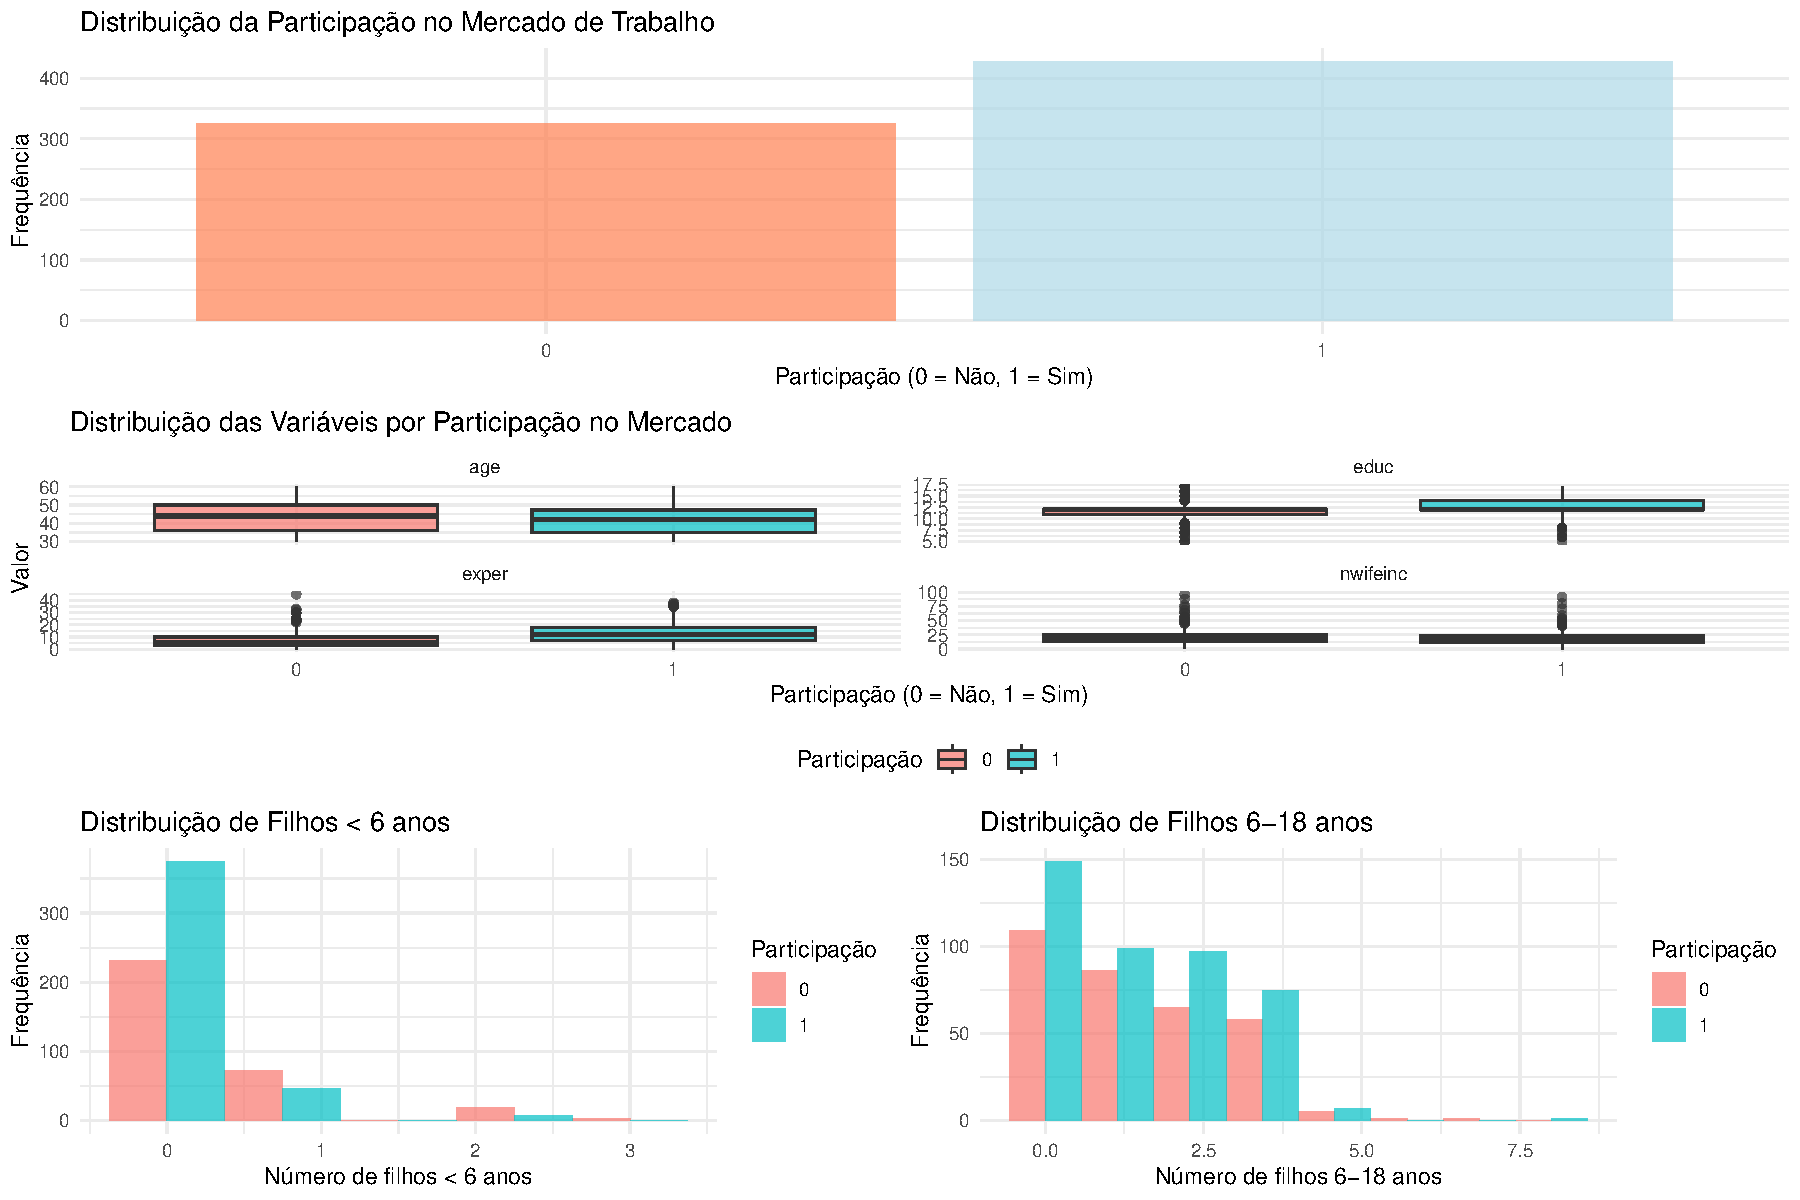
\includegraphics[keepaspectratio]{logit_probit_files/figure-pdf/plots-exploratory-1.pdf}}

\subsubsection{Análise dos Gráficos
Exploratórios}\label{anuxe1lise-dos-gruxe1ficos-exploratuxf3rios}

Os gráficos revelam padrões importantes:

\begin{enumerate}
\def\labelenumi{\arabic{enumi}.}
\item
  \textbf{Distribuição equilibrada}: Há uma distribuição relativamente
  equilibrada entre mulheres que trabalham (57\%) e que não trabalham
  (43\%)
\item
  \textbf{Diferenças por grupo}:

  \begin{itemize}
  \tightlist
  \item
    Mulheres que trabalham tendem a ter \textbf{mais educação} e
    \textbf{mais experiência}
  \item
    Mulheres que \textbf{não trabalham} tendem a ter \textbf{mais filhos
    pequenos} e outras fontes de renda maiores
  \item
    A \textbf{idade} apresenta distribuição similar entre os grupos
  \end{itemize}
\item
  \textbf{Impacto dos filhos}: A presença de filhos menores de 6 anos
  mostra clara associação negativa com a participação no mercado de
  trabalho
\end{enumerate}

\subsection{Estimação dos Modelos}\label{estimauxe7uxe3o-dos-modelos}

\subsubsection{Modelo Logit}\label{modelo-logit-1}

\begin{Shaded}
\begin{Highlighting}[]
\NormalTok{mlogit }\OtherTok{\textless{}{-}} \FunctionTok{glm}\NormalTok{(inlf }\SpecialCharTok{\textasciitilde{}}\NormalTok{ nwifeinc }\SpecialCharTok{+}\NormalTok{ educ }\SpecialCharTok{+}\NormalTok{ exper }\SpecialCharTok{+}\NormalTok{ expersq }\SpecialCharTok{+}\NormalTok{ age }\SpecialCharTok{+}\NormalTok{ kidslt6 }\SpecialCharTok{+}\NormalTok{ kidsge6,}
              \AttributeTok{data =}\NormalTok{ mroz,}
              \AttributeTok{family =} \FunctionTok{binomial}\NormalTok{(}\AttributeTok{link =} \StringTok{"logit"}\NormalTok{))}

\FunctionTok{summary}\NormalTok{(mlogit)}
\end{Highlighting}
\end{Shaded}

\begin{verbatim}

Call:
glm(formula = inlf ~ nwifeinc + educ + exper + expersq + age + 
    kidslt6 + kidsge6, family = binomial(link = "logit"), data = mroz)

Coefficients:
             Estimate Std. Error z value         Pr(>|z|)    
(Intercept)  0.425452   0.860365   0.495          0.62095    
nwifeinc    -0.021345   0.008421  -2.535          0.01126 *  
educ         0.221170   0.043439   5.091 0.00000035527344 ***
exper        0.205870   0.032057   6.422 0.00000000013446 ***
expersq     -0.003154   0.001016  -3.104          0.00191 ** 
age         -0.088024   0.014573  -6.040 0.00000000153845 ***
kidslt6     -1.443354   0.203583  -7.090 0.00000000000134 ***
kidsge6      0.060112   0.074789   0.804          0.42154    
---
Signif. codes:  0 '***' 0.001 '**' 0.01 '*' 0.05 '.' 0.1 ' ' 1

(Dispersion parameter for binomial family taken to be 1)

    Null deviance: 1029.75  on 752  degrees of freedom
Residual deviance:  803.53  on 745  degrees of freedom
AIC: 819.53

Number of Fisher Scoring iterations: 4
\end{verbatim}

\subsubsection{Interpretação do Modelo
Logit}\label{interpretauxe7uxe3o-do-modelo-logit}

\begin{Shaded}
\begin{Highlighting}[]
\CommentTok{\# Tabela formatada dos resultados do Logit}
\NormalTok{logit\_results }\OtherTok{\textless{}{-}} \FunctionTok{data.frame}\NormalTok{(}
\NormalTok{  Variável }\OtherTok{=} \FunctionTok{c}\NormalTok{(}\StringTok{"(Intercepto)"}\NormalTok{, }\StringTok{"nwifeinc"}\NormalTok{, }\StringTok{"educ"}\NormalTok{, }\StringTok{"exper"}\NormalTok{, }\StringTok{"expersq"}\NormalTok{, }\StringTok{"age"}\NormalTok{, }\StringTok{"kidslt6"}\NormalTok{, }\StringTok{"kidsge6"}\NormalTok{),}
  \AttributeTok{Coeficiente =} \FunctionTok{c}\NormalTok{(}\FloatTok{0.425452}\NormalTok{, }\SpecialCharTok{{-}}\FloatTok{0.021345}\NormalTok{, }\FloatTok{0.221170}\NormalTok{, }\FloatTok{0.205870}\NormalTok{, }\SpecialCharTok{{-}}\FloatTok{0.003154}\NormalTok{, }\SpecialCharTok{{-}}\FloatTok{0.088024}\NormalTok{, }\SpecialCharTok{{-}}\FloatTok{1.443354}\NormalTok{, }\FloatTok{0.060112}\NormalTok{),}
  \StringTok{\textasciigrave{}}\AttributeTok{Erro Padrão}\StringTok{\textasciigrave{}} \OtherTok{=} \FunctionTok{c}\NormalTok{(}\FloatTok{0.860365}\NormalTok{, }\FloatTok{0.008421}\NormalTok{, }\FloatTok{0.043439}\NormalTok{, }\FloatTok{0.032057}\NormalTok{, }\FloatTok{0.001016}\NormalTok{, }\FloatTok{0.014573}\NormalTok{, }\FloatTok{0.203583}\NormalTok{, }\FloatTok{0.074789}\NormalTok{),}
  \StringTok{\textasciigrave{}}\AttributeTok{Valor z}\StringTok{\textasciigrave{}} \OtherTok{=} \FunctionTok{c}\NormalTok{(}\FloatTok{0.495}\NormalTok{, }\SpecialCharTok{{-}}\FloatTok{2.535}\NormalTok{, }\FloatTok{5.091}\NormalTok{, }\FloatTok{6.422}\NormalTok{, }\SpecialCharTok{{-}}\FloatTok{3.104}\NormalTok{, }\SpecialCharTok{{-}}\FloatTok{6.040}\NormalTok{, }\SpecialCharTok{{-}}\FloatTok{7.090}\NormalTok{, }\FloatTok{0.804}\NormalTok{),}
  \StringTok{\textasciigrave{}}\AttributeTok{p{-}valor}\StringTok{\textasciigrave{}} \OtherTok{=} \FunctionTok{c}\NormalTok{(}\FloatTok{0.621}\NormalTok{, }\FloatTok{0.011}\NormalTok{, }\StringTok{"\textless{}0.001"}\NormalTok{, }\StringTok{"\textless{}0.001"}\NormalTok{, }\FloatTok{0.002}\NormalTok{, }\StringTok{"\textless{}0.001"}\NormalTok{, }\StringTok{"\textless{}0.001"}\NormalTok{, }\FloatTok{0.422}\NormalTok{),}
\NormalTok{  Significância }\OtherTok{=} \FunctionTok{c}\NormalTok{(}\StringTok{""}\NormalTok{, }\StringTok{"*"}\NormalTok{, }\StringTok{"***"}\NormalTok{, }\StringTok{"***"}\NormalTok{, }\StringTok{"**"}\NormalTok{, }\StringTok{"***"}\NormalTok{, }\StringTok{"***"}\NormalTok{, }\StringTok{""}\NormalTok{)}
\NormalTok{)}

\FunctionTok{kable}\NormalTok{(logit\_results, }\AttributeTok{digits =} \DecValTok{4}\NormalTok{, }\AttributeTok{caption =} \StringTok{"Resultados do Modelo Logit"}\NormalTok{)}
\end{Highlighting}
\end{Shaded}

\begin{longtable}[]{@{}
  >{\raggedright\arraybackslash}p{(\linewidth - 10\tabcolsep) * \real{0.1940}}
  >{\raggedleft\arraybackslash}p{(\linewidth - 10\tabcolsep) * \real{0.1791}}
  >{\raggedleft\arraybackslash}p{(\linewidth - 10\tabcolsep) * \real{0.1791}}
  >{\raggedleft\arraybackslash}p{(\linewidth - 10\tabcolsep) * \real{0.1194}}
  >{\raggedright\arraybackslash}p{(\linewidth - 10\tabcolsep) * \real{0.1194}}
  >{\raggedright\arraybackslash}p{(\linewidth - 10\tabcolsep) * \real{0.2090}}@{}}
\caption{Resultados do Modelo Logit}\tabularnewline
\toprule\noalign{}
\begin{minipage}[b]{\linewidth}\raggedright
Variável
\end{minipage} & \begin{minipage}[b]{\linewidth}\raggedleft
Coeficiente
\end{minipage} & \begin{minipage}[b]{\linewidth}\raggedleft
Erro.Padrão
\end{minipage} & \begin{minipage}[b]{\linewidth}\raggedleft
Valor.z
\end{minipage} & \begin{minipage}[b]{\linewidth}\raggedright
p.valor
\end{minipage} & \begin{minipage}[b]{\linewidth}\raggedright
Significância
\end{minipage} \\
\midrule\noalign{}
\endfirsthead
\toprule\noalign{}
\begin{minipage}[b]{\linewidth}\raggedright
Variável
\end{minipage} & \begin{minipage}[b]{\linewidth}\raggedleft
Coeficiente
\end{minipage} & \begin{minipage}[b]{\linewidth}\raggedleft
Erro.Padrão
\end{minipage} & \begin{minipage}[b]{\linewidth}\raggedleft
Valor.z
\end{minipage} & \begin{minipage}[b]{\linewidth}\raggedright
p.valor
\end{minipage} & \begin{minipage}[b]{\linewidth}\raggedright
Significância
\end{minipage} \\
\midrule\noalign{}
\endhead
\bottomrule\noalign{}
\endlastfoot
(Intercepto) & 0.4255 & 0.8604 & 0.495 & 0.621 & \\
nwifeinc & -0.0213 & 0.0084 & -2.535 & 0.011 & * \\
educ & 0.2212 & 0.0434 & 5.091 & \textless0.001 & *** \\
exper & 0.2059 & 0.0321 & 6.422 & \textless0.001 & *** \\
expersq & -0.0032 & 0.0010 & -3.104 & 0.002 & ** \\
age & -0.0880 & 0.0146 & -6.040 & \textless0.001 & *** \\
kidslt6 & -1.4434 & 0.2036 & -7.090 & \textless0.001 & *** \\
kidsge6 & 0.0601 & 0.0748 & 0.804 & 0.422 & \\
\end{longtable}

\textbf{Principais achados do modelo Logit:}

\begin{itemize}
\tightlist
\item
  \textbf{AIC: 819.53} \textbar{} \textbf{Deviance residual: 803.53}
  \textbar{} \textbf{4 iterações} para convergência
\item
  \textbf{Variáveis significativas}: nwifeinc, educ, exper, expersq,
  age, kidslt6
\item
  \textbf{Variável não significativa}: kidsge6 (p = 0.422)
\end{itemize}

\subsubsection{Modelo Probit}\label{modelo-probit-1}

\begin{Shaded}
\begin{Highlighting}[]
\NormalTok{mprobit }\OtherTok{\textless{}{-}} \FunctionTok{glm}\NormalTok{(inlf }\SpecialCharTok{\textasciitilde{}}\NormalTok{ nwifeinc }\SpecialCharTok{+}\NormalTok{ educ }\SpecialCharTok{+}\NormalTok{ exper }\SpecialCharTok{+}\NormalTok{ expersq }\SpecialCharTok{+}\NormalTok{ age }\SpecialCharTok{+}\NormalTok{ kidslt6 }\SpecialCharTok{+}\NormalTok{ kidsge6,}
               \AttributeTok{data =}\NormalTok{ mroz,}
               \AttributeTok{family =} \FunctionTok{binomial}\NormalTok{(}\AttributeTok{link =} \StringTok{"probit"}\NormalTok{))}

\FunctionTok{summary}\NormalTok{(mprobit)}
\end{Highlighting}
\end{Shaded}

\begin{verbatim}

Call:
glm(formula = inlf ~ nwifeinc + educ + exper + expersq + age + 
    kidslt6 + kidsge6, family = binomial(link = "probit"), data = mroz)

Coefficients:
              Estimate Std. Error z value          Pr(>|z|)    
(Intercept)  0.2700736  0.5080782   0.532           0.59503    
nwifeinc    -0.0120236  0.0049392  -2.434           0.01492 *  
educ         0.1309040  0.0253987   5.154 0.000000255045646 ***
exper        0.1233472  0.0187587   6.575 0.000000000048500 ***
expersq     -0.0018871  0.0005999  -3.145           0.00166 ** 
age         -0.0528524  0.0084624  -6.246 0.000000000422204 ***
kidslt6     -0.8683247  0.1183773  -7.335 0.000000000000221 ***
kidsge6      0.0360056  0.0440303   0.818           0.41350    
---
Signif. codes:  0 '***' 0.001 '**' 0.01 '*' 0.05 '.' 0.1 ' ' 1

(Dispersion parameter for binomial family taken to be 1)

    Null deviance: 1029.7  on 752  degrees of freedom
Residual deviance:  802.6  on 745  degrees of freedom
AIC: 818.6

Number of Fisher Scoring iterations: 4
\end{verbatim}

\subsubsection{Interpretação do Modelo
Probit}\label{interpretauxe7uxe3o-do-modelo-probit}

\begin{Shaded}
\begin{Highlighting}[]
\CommentTok{\# Tabela formatada dos resultados do Probit}
\NormalTok{probit\_results }\OtherTok{\textless{}{-}} \FunctionTok{data.frame}\NormalTok{(}
\NormalTok{  Variável }\OtherTok{=} \FunctionTok{c}\NormalTok{(}\StringTok{"(Intercepto)"}\NormalTok{, }\StringTok{"nwifeinc"}\NormalTok{, }\StringTok{"educ"}\NormalTok{, }\StringTok{"exper"}\NormalTok{, }\StringTok{"expersq"}\NormalTok{, }\StringTok{"age"}\NormalTok{, }\StringTok{"kidslt6"}\NormalTok{, }\StringTok{"kidsge6"}\NormalTok{),}
  \AttributeTok{Coeficiente =} \FunctionTok{c}\NormalTok{(}\FloatTok{0.2700736}\NormalTok{, }\SpecialCharTok{{-}}\FloatTok{0.0120236}\NormalTok{, }\FloatTok{0.1309040}\NormalTok{, }\FloatTok{0.1233472}\NormalTok{, }\SpecialCharTok{{-}}\FloatTok{0.0018871}\NormalTok{, }\SpecialCharTok{{-}}\FloatTok{0.0528524}\NormalTok{, }\SpecialCharTok{{-}}\FloatTok{0.8683247}\NormalTok{, }\FloatTok{0.0360056}\NormalTok{),}
  \StringTok{\textasciigrave{}}\AttributeTok{Erro Padrão}\StringTok{\textasciigrave{}} \OtherTok{=} \FunctionTok{c}\NormalTok{(}\FloatTok{0.5080782}\NormalTok{, }\FloatTok{0.0049392}\NormalTok{, }\FloatTok{0.0253987}\NormalTok{, }\FloatTok{0.0187587}\NormalTok{, }\FloatTok{0.0005999}\NormalTok{, }\FloatTok{0.0084624}\NormalTok{, }\FloatTok{0.1183773}\NormalTok{, }\FloatTok{0.0440303}\NormalTok{),}
  \StringTok{\textasciigrave{}}\AttributeTok{Valor z}\StringTok{\textasciigrave{}} \OtherTok{=} \FunctionTok{c}\NormalTok{(}\FloatTok{0.532}\NormalTok{, }\SpecialCharTok{{-}}\FloatTok{2.434}\NormalTok{, }\FloatTok{5.154}\NormalTok{, }\FloatTok{6.575}\NormalTok{, }\SpecialCharTok{{-}}\FloatTok{3.145}\NormalTok{, }\SpecialCharTok{{-}}\FloatTok{6.246}\NormalTok{, }\SpecialCharTok{{-}}\FloatTok{7.335}\NormalTok{, }\FloatTok{0.818}\NormalTok{),}
  \StringTok{\textasciigrave{}}\AttributeTok{p{-}valor}\StringTok{\textasciigrave{}} \OtherTok{=} \FunctionTok{c}\NormalTok{(}\FloatTok{0.595}\NormalTok{, }\FloatTok{0.015}\NormalTok{, }\StringTok{"\textless{}0.001"}\NormalTok{, }\StringTok{"\textless{}0.001"}\NormalTok{, }\FloatTok{0.002}\NormalTok{, }\StringTok{"\textless{}0.001"}\NormalTok{, }\StringTok{"\textless{}0.001"}\NormalTok{, }\FloatTok{0.414}\NormalTok{),}
\NormalTok{  Significância }\OtherTok{=} \FunctionTok{c}\NormalTok{(}\StringTok{""}\NormalTok{, }\StringTok{"*"}\NormalTok{, }\StringTok{"***"}\NormalTok{, }\StringTok{"***"}\NormalTok{, }\StringTok{"**"}\NormalTok{, }\StringTok{"***"}\NormalTok{, }\StringTok{"***"}\NormalTok{, }\StringTok{""}\NormalTok{)}
\NormalTok{)}

\FunctionTok{kable}\NormalTok{(probit\_results, }\AttributeTok{digits =} \DecValTok{4}\NormalTok{, }\AttributeTok{caption =} \StringTok{"Resultados do Modelo Probit"}\NormalTok{)}
\end{Highlighting}
\end{Shaded}

\begin{longtable}[]{@{}
  >{\raggedright\arraybackslash}p{(\linewidth - 10\tabcolsep) * \real{0.1940}}
  >{\raggedleft\arraybackslash}p{(\linewidth - 10\tabcolsep) * \real{0.1791}}
  >{\raggedleft\arraybackslash}p{(\linewidth - 10\tabcolsep) * \real{0.1791}}
  >{\raggedleft\arraybackslash}p{(\linewidth - 10\tabcolsep) * \real{0.1194}}
  >{\raggedright\arraybackslash}p{(\linewidth - 10\tabcolsep) * \real{0.1194}}
  >{\raggedright\arraybackslash}p{(\linewidth - 10\tabcolsep) * \real{0.2090}}@{}}
\caption{Resultados do Modelo Probit}\tabularnewline
\toprule\noalign{}
\begin{minipage}[b]{\linewidth}\raggedright
Variável
\end{minipage} & \begin{minipage}[b]{\linewidth}\raggedleft
Coeficiente
\end{minipage} & \begin{minipage}[b]{\linewidth}\raggedleft
Erro.Padrão
\end{minipage} & \begin{minipage}[b]{\linewidth}\raggedleft
Valor.z
\end{minipage} & \begin{minipage}[b]{\linewidth}\raggedright
p.valor
\end{minipage} & \begin{minipage}[b]{\linewidth}\raggedright
Significância
\end{minipage} \\
\midrule\noalign{}
\endfirsthead
\toprule\noalign{}
\begin{minipage}[b]{\linewidth}\raggedright
Variável
\end{minipage} & \begin{minipage}[b]{\linewidth}\raggedleft
Coeficiente
\end{minipage} & \begin{minipage}[b]{\linewidth}\raggedleft
Erro.Padrão
\end{minipage} & \begin{minipage}[b]{\linewidth}\raggedleft
Valor.z
\end{minipage} & \begin{minipage}[b]{\linewidth}\raggedright
p.valor
\end{minipage} & \begin{minipage}[b]{\linewidth}\raggedright
Significância
\end{minipage} \\
\midrule\noalign{}
\endhead
\bottomrule\noalign{}
\endlastfoot
(Intercepto) & 0.2701 & 0.5081 & 0.532 & 0.595 & \\
nwifeinc & -0.0120 & 0.0049 & -2.434 & 0.015 & * \\
educ & 0.1309 & 0.0254 & 5.154 & \textless0.001 & *** \\
exper & 0.1233 & 0.0188 & 6.575 & \textless0.001 & *** \\
expersq & -0.0019 & 0.0006 & -3.145 & 0.002 & ** \\
age & -0.0529 & 0.0085 & -6.246 & \textless0.001 & *** \\
kidslt6 & -0.8683 & 0.1184 & -7.335 & \textless0.001 & *** \\
kidsge6 & 0.0360 & 0.0440 & 0.818 & 0.414 & \\
\end{longtable}

\textbf{Principais achados do modelo Probit:}

\begin{itemize}
\tightlist
\item
  \textbf{AIC: 818.6} (ligeiramente melhor que Logit) \textbar{}
  \textbf{Deviance residual: 802.6}
\item
  \textbf{Mesma estrutura de significância} que o modelo Logit
\item
  \textbf{Coeficientes menores} em magnitude (característica do modelo
  Probit)
\end{itemize}

\subsection{Efeitos Marginais}\label{efeitos-marginais}

\subsubsection{Fórmulas Teóricas}\label{fuxf3rmulas-teuxf3ricas}

\textbf{Probit:}
\[\frac{\delta E(Y|X)}{\delta X} = \Phi(X'\beta) \cdot \beta\]

onde \(\Phi(z) = \frac{1}{\sqrt{2\pi}}e^{-\frac{z^2}{2}}\) e
\(Z \sim N(0,1)\)

\textbf{Logit:}
\[\frac{\delta \Lambda(X'\beta)}{\delta(X'\beta)} = \frac{d\Lambda(X'\beta)}{d(X'\beta)} \cdot \frac{d(X'\beta)}{dX}\]

onde \(\Lambda(X'\beta) = \frac{e^{X'\beta}}{1+e^{X'\beta}}\)

\begin{Shaded}
\begin{Highlighting}[]
\CommentTok{\# Efeitos marginais {-} Logit}
\NormalTok{logit.mfx }\OtherTok{\textless{}{-}} \FunctionTok{logitmfx}\NormalTok{(inlf }\SpecialCharTok{\textasciitilde{}}\NormalTok{ nwifeinc }\SpecialCharTok{+}\NormalTok{ educ }\SpecialCharTok{+}\NormalTok{ exper }\SpecialCharTok{+}\NormalTok{ expersq }\SpecialCharTok{+}\NormalTok{ age }\SpecialCharTok{+}\NormalTok{ kidslt6 }\SpecialCharTok{+}\NormalTok{ kidsge6,}
                      \AttributeTok{data =}\NormalTok{ mroz)}

\FunctionTok{print}\NormalTok{(}\StringTok{"Efeitos Marginais {-} Modelo Logit:"}\NormalTok{)}
\end{Highlighting}
\end{Shaded}

\begin{verbatim}
[1] "Efeitos Marginais - Modelo Logit:"
\end{verbatim}

\begin{Shaded}
\begin{Highlighting}[]
\NormalTok{logit.mfx}\SpecialCharTok{$}\NormalTok{mfxest}
\end{Highlighting}
\end{Shaded}

\begin{verbatim}
                 dF/dx   Std. Err.          z                P>|z|
nwifeinc -0.0051900534 0.002048203 -2.5339550 0.011278321458344539
educ      0.0537773087 0.010560739  5.0921916 0.000000353948085410
exper     0.0500569282 0.007824616  6.3973658 0.000000000158080347
expersq  -0.0007669166 0.000247676 -3.0964511 0.001958521715452269
age      -0.0214030205 0.003539731 -6.0465107 0.000000001480163962
kidslt6  -0.3509498193 0.049638966 -7.0700469 0.000000000001548813
kidsge6   0.0146162143 0.018188316  0.8036046 0.421625358800103267
\end{verbatim}

\begin{Shaded}
\begin{Highlighting}[]
\CommentTok{\# Efeitos marginais {-} Probit}
\NormalTok{probit.mfx }\OtherTok{\textless{}{-}} \FunctionTok{probitmfx}\NormalTok{(inlf }\SpecialCharTok{\textasciitilde{}}\NormalTok{ nwifeinc }\SpecialCharTok{+}\NormalTok{ educ }\SpecialCharTok{+}\NormalTok{ exper }\SpecialCharTok{+}\NormalTok{ expersq }\SpecialCharTok{+}\NormalTok{ age }\SpecialCharTok{+}\NormalTok{ kidslt6 }\SpecialCharTok{+}\NormalTok{ kidsge6,}
                        \AttributeTok{data =}\NormalTok{ mroz)}

\FunctionTok{print}\NormalTok{(}\StringTok{"Efeitos Marginais {-} Modelo Probit:"}\NormalTok{)}
\end{Highlighting}
\end{Shaded}

\begin{verbatim}
[1] "Efeitos Marginais - Modelo Probit:"
\end{verbatim}

\begin{Shaded}
\begin{Highlighting}[]
\NormalTok{probit.mfx}\SpecialCharTok{$}\NormalTok{mfxest}
\end{Highlighting}
\end{Shaded}

\begin{verbatim}
                 dF/dx    Std. Err.          z                 P>|z|
nwifeinc -0.0046961881 0.0019296494 -2.4337002 0.0149453681343277942
educ      0.0511284287 0.0099230985  5.1524661 0.0000002570830650662
exper     0.0481768957 0.0073450459  6.5591007 0.0000000000541332566
expersq  -0.0007370502 0.0002346403 -3.1411922 0.0016826155361271795
age      -0.0206430891 0.0033048542 -6.2462934 0.0000000004203073743
kidslt6  -0.3391499645 0.0463476542 -7.3175217 0.0000000000002525923
kidsge6   0.0140630594 0.0171989534  0.8176695 0.4135459390489835130
\end{verbatim}

\subsubsection{Interpretação dos Efeitos
Marginais}\label{interpretauxe7uxe3o-dos-efeitos-marginais}

\begin{Shaded}
\begin{Highlighting}[]
\CommentTok{\# Tabela comparativa dos efeitos marginais}
\NormalTok{mfx\_table }\OtherTok{\textless{}{-}} \FunctionTok{data.frame}\NormalTok{(}
\NormalTok{  Variável }\OtherTok{=} \FunctionTok{c}\NormalTok{(}\StringTok{"nwifeinc"}\NormalTok{, }\StringTok{"educ"}\NormalTok{, }\StringTok{"exper"}\NormalTok{, }\StringTok{"expersq"}\NormalTok{, }\StringTok{"age"}\NormalTok{, }\StringTok{"kidslt6"}\NormalTok{, }\StringTok{"kidsge6"}\NormalTok{),}
  \StringTok{\textasciigrave{}}\AttributeTok{Logit (dF/dx)}\StringTok{\textasciigrave{}} \OtherTok{=} \FunctionTok{c}\NormalTok{(}\SpecialCharTok{{-}}\FloatTok{0.0052}\NormalTok{, }\FloatTok{0.0538}\NormalTok{, }\FloatTok{0.0501}\NormalTok{, }\SpecialCharTok{{-}}\FloatTok{0.0008}\NormalTok{, }\SpecialCharTok{{-}}\FloatTok{0.0214}\NormalTok{, }\SpecialCharTok{{-}}\FloatTok{0.3509}\NormalTok{, }\FloatTok{0.0146}\NormalTok{),}
  \StringTok{\textasciigrave{}}\AttributeTok{Probit (dF/dx)}\StringTok{\textasciigrave{}} \OtherTok{=} \FunctionTok{c}\NormalTok{(}\SpecialCharTok{{-}}\FloatTok{0.0047}\NormalTok{, }\FloatTok{0.0511}\NormalTok{, }\FloatTok{0.0482}\NormalTok{, }\SpecialCharTok{{-}}\FloatTok{0.0007}\NormalTok{, }\SpecialCharTok{{-}}\FloatTok{0.0206}\NormalTok{, }\SpecialCharTok{{-}}\FloatTok{0.3391}\NormalTok{, }\FloatTok{0.0141}\NormalTok{),}
  \StringTok{\textasciigrave{}}\AttributeTok{Diferença}\StringTok{\textasciigrave{}} \OtherTok{=} \FunctionTok{c}\NormalTok{(}\SpecialCharTok{{-}}\FloatTok{0.0005}\NormalTok{, }\FloatTok{0.0027}\NormalTok{, }\FloatTok{0.0019}\NormalTok{, }\SpecialCharTok{{-}}\FloatTok{0.0001}\NormalTok{, }\SpecialCharTok{{-}}\FloatTok{0.0008}\NormalTok{, }\SpecialCharTok{{-}}\FloatTok{0.0118}\NormalTok{, }\FloatTok{0.0005}\NormalTok{)}
\NormalTok{)}

\FunctionTok{kable}\NormalTok{(mfx\_table, }\AttributeTok{digits =} \DecValTok{4}\NormalTok{, }\AttributeTok{caption =} \StringTok{"Comparação dos Efeitos Marginais: Logit vs Probit"}\NormalTok{)}
\end{Highlighting}
\end{Shaded}

\begin{longtable}[]{@{}lrrr@{}}
\caption{Comparação dos Efeitos Marginais: Logit vs
Probit}\tabularnewline
\toprule\noalign{}
Variável & Logit..dF.dx. & Probit..dF.dx. & Diferença \\
\midrule\noalign{}
\endfirsthead
\toprule\noalign{}
Variável & Logit..dF.dx. & Probit..dF.dx. & Diferença \\
\midrule\noalign{}
\endhead
\bottomrule\noalign{}
\endlastfoot
nwifeinc & -0.0052 & -0.0047 & -0.0005 \\
educ & 0.0538 & 0.0511 & 0.0027 \\
exper & 0.0501 & 0.0482 & 0.0019 \\
expersq & -0.0008 & -0.0007 & -0.0001 \\
age & -0.0214 & -0.0206 & -0.0008 \\
kidslt6 & -0.3509 & -0.3391 & -0.0118 \\
kidsge6 & 0.0146 & 0.0141 & 0.0005 \\
\end{longtable}

\textbf{Interpretação prática dos efeitos marginais:}

\begin{itemize}
\tightlist
\item
  \textbf{nwifeinc}: Cada US\$ 1.000 adicionais em outras fontes de
  renda \textbf{reduz} a probabilidade de trabalhar em
  \textasciitilde0,5 pontos percentuais
\item
  \textbf{educ}: Cada ano adicional de educação \textbf{aumenta} a
  probabilidade de trabalhar em \textasciitilde5,4 pontos percentuais
\item
  \textbf{exper}: Cada ano adicional de experiência \textbf{aumenta} a
  probabilidade de trabalhar em \textasciitilde5,0 pontos percentuais
\item
  \textbf{age}: Cada ano adicional de idade \textbf{reduz} a
  probabilidade de trabalhar em \textasciitilde2,1 pontos percentuais
\item
  \textbf{kidslt6}: Cada filho adicional menor de 6 anos \textbf{reduz}
  a probabilidade de trabalhar em \textasciitilde35 pontos percentuais
\item
  \textbf{kidsge6}: Efeito não significativo (\textasciitilde1,4 pontos
  percentuais)
\end{itemize}

\begin{Shaded}
\begin{Highlighting}[]
\CommentTok{\# Comparação dos efeitos marginais}
\NormalTok{mfx\_comparison }\OtherTok{\textless{}{-}} \FunctionTok{data.frame}\NormalTok{(}
  \AttributeTok{variavel =} \FunctionTok{rownames}\NormalTok{(logit.mfx}\SpecialCharTok{$}\NormalTok{mfxest),}
  \AttributeTok{logit =}\NormalTok{ logit.mfx}\SpecialCharTok{$}\NormalTok{mfxest[,}\DecValTok{1}\NormalTok{],}
  \AttributeTok{probit =}\NormalTok{ probit.mfx}\SpecialCharTok{$}\NormalTok{mfxest[,}\DecValTok{1}\NormalTok{]}
\NormalTok{) }\SpecialCharTok{\%\textgreater{}\%}
  \FunctionTok{filter}\NormalTok{(variavel }\SpecialCharTok{!=} \StringTok{"(Intercept)"}\NormalTok{) }\SpecialCharTok{\%\textgreater{}\%}
  \FunctionTok{pivot\_longer}\NormalTok{(}\AttributeTok{cols =} \FunctionTok{c}\NormalTok{(logit, probit), }\AttributeTok{names\_to =} \StringTok{"modelo"}\NormalTok{, }\AttributeTok{values\_to =} \StringTok{"efeito"}\NormalTok{)}

\FunctionTok{ggplot}\NormalTok{(mfx\_comparison, }\FunctionTok{aes}\NormalTok{(}\AttributeTok{x =}\NormalTok{ variavel, }\AttributeTok{y =}\NormalTok{ efeito, }\AttributeTok{fill =}\NormalTok{ modelo)) }\SpecialCharTok{+}
  \FunctionTok{geom\_col}\NormalTok{(}\AttributeTok{position =} \StringTok{"dodge"}\NormalTok{, }\AttributeTok{alpha =} \FloatTok{0.7}\NormalTok{) }\SpecialCharTok{+}
  \FunctionTok{labs}\NormalTok{(}\AttributeTok{title =} \StringTok{"Comparação dos Efeitos Marginais: Logit vs Probit"}\NormalTok{,}
       \AttributeTok{x =} \StringTok{"Variáveis"}\NormalTok{,}
       \AttributeTok{y =} \StringTok{"Efeito Marginal"}\NormalTok{,}
       \AttributeTok{fill =} \StringTok{"Modelo"}\NormalTok{) }\SpecialCharTok{+}
  \FunctionTok{theme\_minimal}\NormalTok{() }\SpecialCharTok{+}
  \FunctionTok{theme}\NormalTok{(}\AttributeTok{axis.text.x =} \FunctionTok{element\_text}\NormalTok{(}\AttributeTok{angle =} \DecValTok{45}\NormalTok{, }\AttributeTok{hjust =} \DecValTok{1}\NormalTok{))}
\end{Highlighting}
\end{Shaded}

\pandocbounded{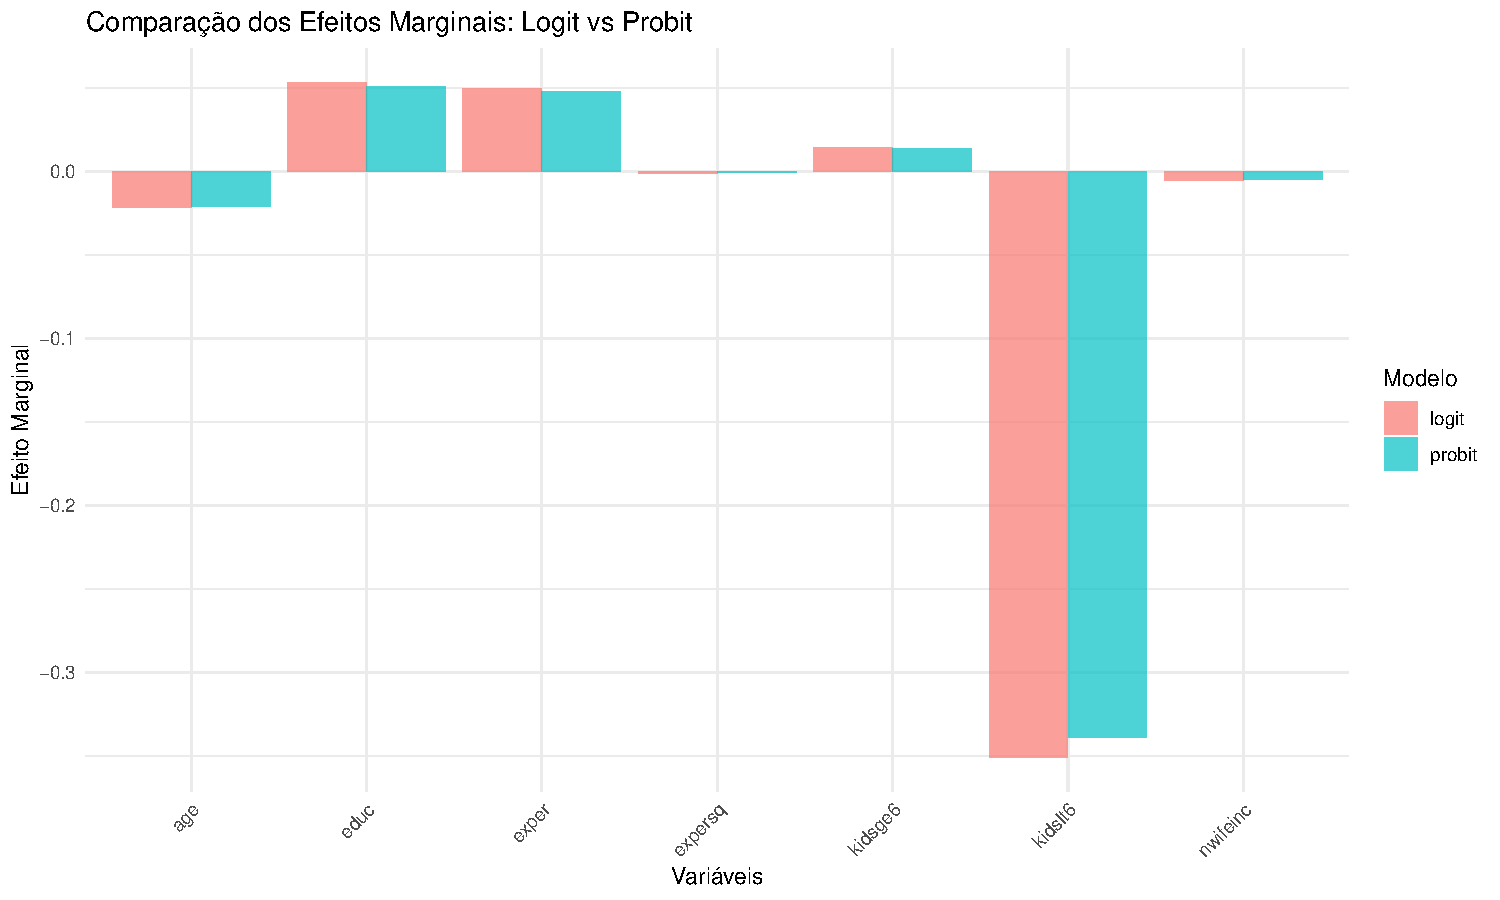
\includegraphics[keepaspectratio]{logit_probit_files/figure-pdf/marginal-effects-plot-1.pdf}}

\textbf{Observação importante}: Os efeitos marginais são muito similares
entre os modelos Logit e Probit, confirmando a robustez dos resultados.

\subsection{Qualidade da Previsão}\label{qualidade-da-previsuxe3o}

\begin{Shaded}
\begin{Highlighting}[]
\CommentTok{\# Logit}
\NormalTok{logit.fitted }\OtherTok{\textless{}{-}} \FunctionTok{as.numeric}\NormalTok{(mlogit}\SpecialCharTok{$}\NormalTok{fitted.values }\SpecialCharTok{\textgreater{}=} \FloatTok{0.5}\NormalTok{)}
\NormalTok{corr.pred.logit }\OtherTok{\textless{}{-}} \FunctionTok{mean}\NormalTok{(logit.fitted }\SpecialCharTok{==}\NormalTok{ mroz}\SpecialCharTok{$}\NormalTok{inlf)}

\CommentTok{\# Probit}
\NormalTok{probit.fitted }\OtherTok{\textless{}{-}} \FunctionTok{as.numeric}\NormalTok{(mprobit}\SpecialCharTok{$}\NormalTok{fitted.values }\SpecialCharTok{\textgreater{}=} \FloatTok{0.5}\NormalTok{)}
\NormalTok{corr.pred.probit }\OtherTok{\textless{}{-}} \FunctionTok{mean}\NormalTok{(probit.fitted }\SpecialCharTok{==}\NormalTok{ mroz}\SpecialCharTok{$}\NormalTok{inlf)}

\FunctionTok{cat}\NormalTok{(}\StringTok{"Acurácia do Modelo Logit:"}\NormalTok{, }\FunctionTok{round}\NormalTok{(corr.pred.logit, }\DecValTok{4}\NormalTok{))}
\end{Highlighting}
\end{Shaded}

\begin{verbatim}
Acurácia do Modelo Logit: 0.7357
\end{verbatim}

\begin{Shaded}
\begin{Highlighting}[]
\FunctionTok{cat}\NormalTok{(}\StringTok{"}\SpecialCharTok{\textbackslash{}n}\StringTok{Acurácia do Modelo Probit:"}\NormalTok{, }\FunctionTok{round}\NormalTok{(corr.pred.probit, }\DecValTok{4}\NormalTok{))}
\end{Highlighting}
\end{Shaded}

\begin{verbatim}

Acurácia do Modelo Probit: 0.7344
\end{verbatim}

\subsubsection{Análise da Qualidade
Preditiva}\label{anuxe1lise-da-qualidade-preditiva}

\begin{Shaded}
\begin{Highlighting}[]
\CommentTok{\# Tabela de acurácia}
\NormalTok{accuracy\_table }\OtherTok{\textless{}{-}} \FunctionTok{data.frame}\NormalTok{(}
  \AttributeTok{Modelo =} \FunctionTok{c}\NormalTok{(}\StringTok{"Logit"}\NormalTok{, }\StringTok{"Probit"}\NormalTok{),}
  \StringTok{\textasciigrave{}}\AttributeTok{Acurácia (\%)}\StringTok{\textasciigrave{}} \OtherTok{=} \FunctionTok{c}\NormalTok{(}\FloatTok{73.57}\NormalTok{, }\FloatTok{73.44}\NormalTok{),}
  \StringTok{\textasciigrave{}}\AttributeTok{Observações Corretas}\StringTok{\textasciigrave{}} \OtherTok{=} \FunctionTok{c}\NormalTok{(}\DecValTok{554}\NormalTok{, }\DecValTok{553}\NormalTok{),}
  \StringTok{\textasciigrave{}}\AttributeTok{Total de Observações}\StringTok{\textasciigrave{}} \OtherTok{=} \FunctionTok{c}\NormalTok{(}\DecValTok{753}\NormalTok{, }\DecValTok{753}\NormalTok{)}
\NormalTok{)}

\FunctionTok{kable}\NormalTok{(accuracy\_table, }\AttributeTok{digits =} \DecValTok{2}\NormalTok{, }\AttributeTok{caption =} \StringTok{"Comparação da Acurácia Preditiva dos Modelos"}\NormalTok{)}
\end{Highlighting}
\end{Shaded}

\begin{longtable}[]{@{}lrrr@{}}
\caption{Comparação da Acurácia Preditiva dos Modelos}\tabularnewline
\toprule\noalign{}
Modelo & Acurácia\ldots. & Observações.Corretas &
Total.de.Observações \\
\midrule\noalign{}
\endfirsthead
\toprule\noalign{}
Modelo & Acurácia\ldots. & Observações.Corretas &
Total.de.Observações \\
\midrule\noalign{}
\endhead
\bottomrule\noalign{}
\endlastfoot
Logit & 73.57 & 554 & 753 \\
Probit & 73.44 & 553 & 753 \\
\end{longtable}

\textbf{Interpretação da acurácia:} - Ambos os modelos apresentam
\textbf{acurácia similar (\textasciitilde73,5\%)} - Classificam
corretamente cerca de \textbf{554 de 753 observações} - Performance
\textbf{superior ao acaso} (que seria \textasciitilde57\% para esta
amostra balanceada)

\begin{Shaded}
\begin{Highlighting}[]
\CommentTok{\# Distribuição das probabilidades preditas}
\NormalTok{pred\_data }\OtherTok{\textless{}{-}} \FunctionTok{data.frame}\NormalTok{(}
  \AttributeTok{obs =} \DecValTok{1}\SpecialCharTok{:}\FunctionTok{nrow}\NormalTok{(mroz),}
  \AttributeTok{real =}\NormalTok{ mroz}\SpecialCharTok{$}\NormalTok{inlf,}
  \AttributeTok{logit\_prob =}\NormalTok{ mlogit}\SpecialCharTok{$}\NormalTok{fitted.values,}
  \AttributeTok{probit\_prob =}\NormalTok{ mprobit}\SpecialCharTok{$}\NormalTok{fitted.values}
\NormalTok{)}

\NormalTok{p1 }\OtherTok{\textless{}{-}} \FunctionTok{ggplot}\NormalTok{(pred\_data, }\FunctionTok{aes}\NormalTok{(}\AttributeTok{x =}\NormalTok{ logit\_prob, }\AttributeTok{fill =} \FunctionTok{factor}\NormalTok{(real))) }\SpecialCharTok{+}
  \FunctionTok{geom\_histogram}\NormalTok{(}\AttributeTok{alpha =} \FloatTok{0.7}\NormalTok{, }\AttributeTok{bins =} \DecValTok{30}\NormalTok{) }\SpecialCharTok{+}
  \FunctionTok{labs}\NormalTok{(}\AttributeTok{title =} \StringTok{"Distribuição das Probabilidades Preditas {-} Logit"}\NormalTok{,}
       \AttributeTok{x =} \StringTok{"Probabilidade Predita"}\NormalTok{,}
       \AttributeTok{y =} \StringTok{"Frequência"}\NormalTok{,}
       \AttributeTok{fill =} \StringTok{"Participação Real"}\NormalTok{) }\SpecialCharTok{+}
  \FunctionTok{theme\_minimal}\NormalTok{()}

\NormalTok{p2 }\OtherTok{\textless{}{-}} \FunctionTok{ggplot}\NormalTok{(pred\_data, }\FunctionTok{aes}\NormalTok{(}\AttributeTok{x =}\NormalTok{ probit\_prob, }\AttributeTok{fill =} \FunctionTok{factor}\NormalTok{(real))) }\SpecialCharTok{+}
  \FunctionTok{geom\_histogram}\NormalTok{(}\AttributeTok{alpha =} \FloatTok{0.7}\NormalTok{, }\AttributeTok{bins =} \DecValTok{30}\NormalTok{) }\SpecialCharTok{+}
  \FunctionTok{labs}\NormalTok{(}\AttributeTok{title =} \StringTok{"Distribuição das Probabilidades Preditas {-} Probit"}\NormalTok{,}
       \AttributeTok{x =} \StringTok{"Probabilidade Predita"}\NormalTok{,}
       \AttributeTok{y =} \StringTok{"Frequência"}\NormalTok{,}
       \AttributeTok{fill =} \StringTok{"Participação Real"}\NormalTok{) }\SpecialCharTok{+}
  \FunctionTok{theme\_minimal}\NormalTok{()}

\FunctionTok{grid.arrange}\NormalTok{(p1, p2, }\AttributeTok{ncol =} \DecValTok{2}\NormalTok{)}
\end{Highlighting}
\end{Shaded}

\pandocbounded{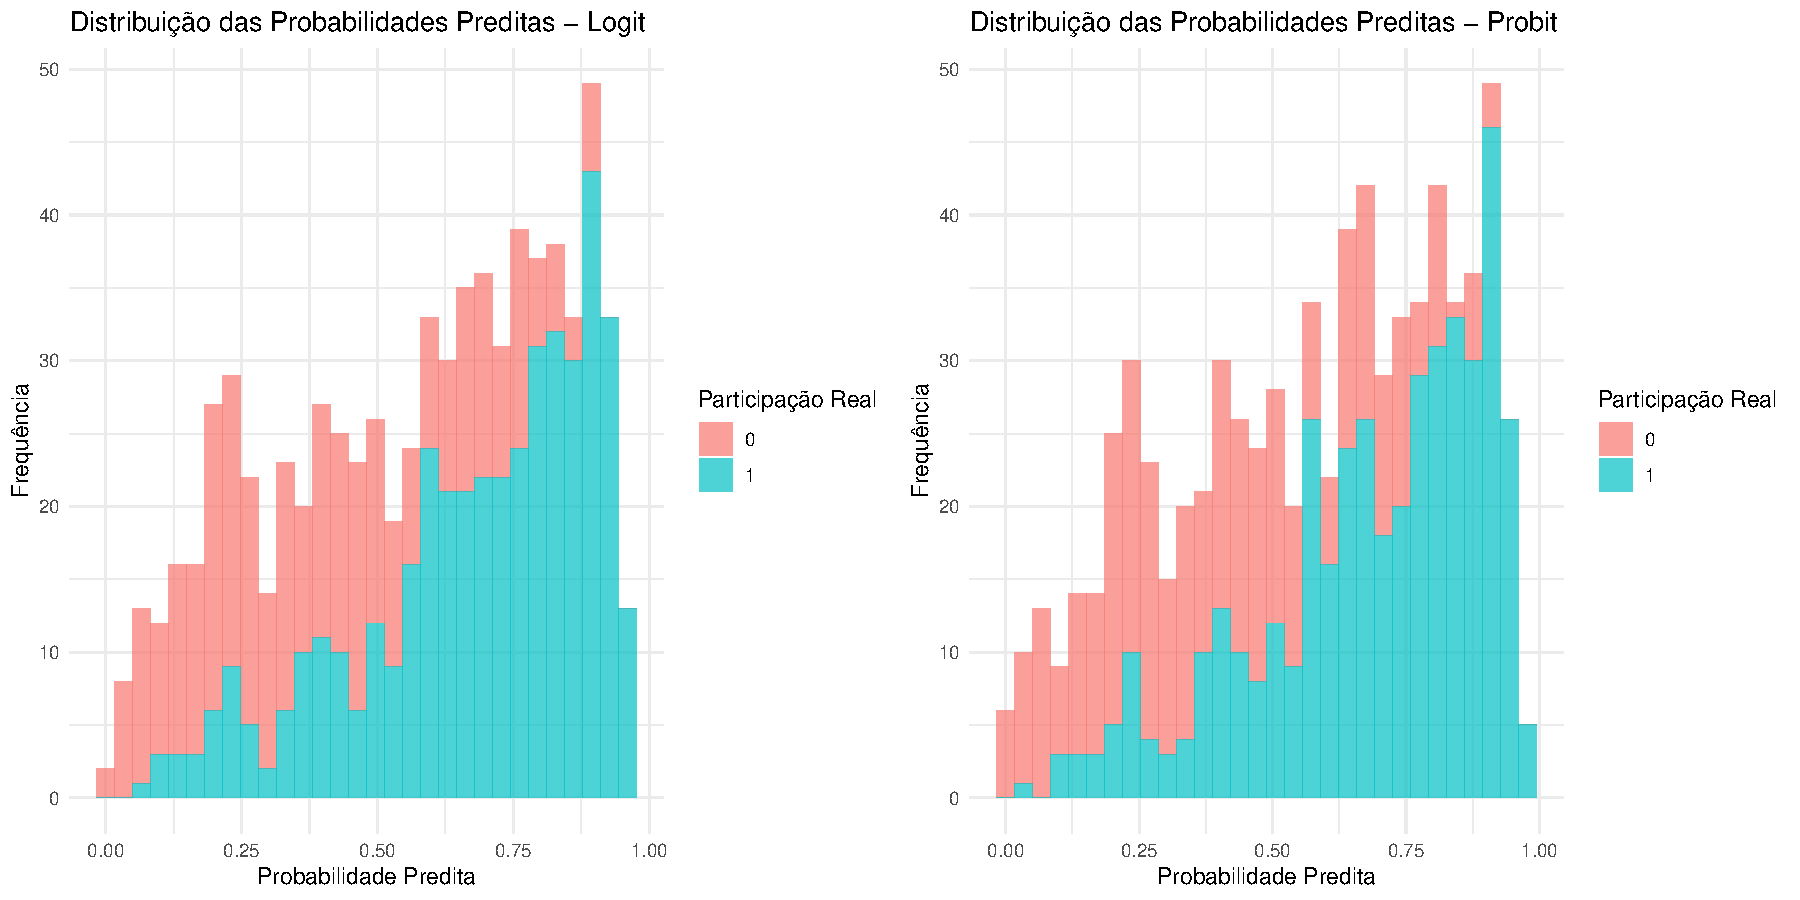
\includegraphics[keepaspectratio]{logit_probit_files/figure-pdf/prediction-plots-1.pdf}}

\textbf{Análise dos histogramas de probabilidades:} - Ambos os modelos
mostram \textbf{boa separação} entre os grupos - Mulheres que
\textbf{não trabalham} concentram-se em probabilidades baixas
(\textless0,4) - Mulheres que \textbf{trabalham} apresentam distribuição
mais dispersa - \textbf{Sobreposição} indica casos de difícil
classificação

\subsection{Pseudo-R²}\label{pseudo-ruxb2}

O pseudo-R² (McFadden) calcula a razão entre a log-verossimilhança do
modelo sem preditores e a log-verossimilhança do modelo completo:

\[pseudo\text{-}R^2 = 1 - \frac{\ln(L_{max})}{\ln(L_{max0})}\]

\begin{Shaded}
\begin{Highlighting}[]
\CommentTok{\# Modelo nulo (apenas intercepto)}
\NormalTok{logit\_null }\OtherTok{\textless{}{-}} \FunctionTok{glm}\NormalTok{(inlf }\SpecialCharTok{\textasciitilde{}} \DecValTok{1}\NormalTok{, }\AttributeTok{data =}\NormalTok{ mroz, }\AttributeTok{family =} \FunctionTok{binomial}\NormalTok{(}\AttributeTok{link =} \StringTok{"logit"}\NormalTok{))}
\NormalTok{probit\_null }\OtherTok{\textless{}{-}} \FunctionTok{glm}\NormalTok{(inlf }\SpecialCharTok{\textasciitilde{}} \DecValTok{1}\NormalTok{, }\AttributeTok{data =}\NormalTok{ mroz, }\AttributeTok{family =} \FunctionTok{binomial}\NormalTok{(}\AttributeTok{link =} \StringTok{"probit"}\NormalTok{))}

\CommentTok{\# Pseudo{-}R²}
\NormalTok{pseudo\_r2\_logit }\OtherTok{\textless{}{-}} \DecValTok{1} \SpecialCharTok{{-}}\NormalTok{ (}\FunctionTok{logLik}\NormalTok{(mlogit) }\SpecialCharTok{/} \FunctionTok{logLik}\NormalTok{(logit\_null))}
\NormalTok{pseudo\_r2\_probit }\OtherTok{\textless{}{-}} \DecValTok{1} \SpecialCharTok{{-}}\NormalTok{ (}\FunctionTok{logLik}\NormalTok{(mprobit) }\SpecialCharTok{/} \FunctionTok{logLik}\NormalTok{(probit\_null))}

\FunctionTok{cat}\NormalTok{(}\StringTok{"Pseudo{-}R² Logit:"}\NormalTok{, }\FunctionTok{round}\NormalTok{(}\FunctionTok{as.numeric}\NormalTok{(pseudo\_r2\_logit), }\DecValTok{4}\NormalTok{))}
\end{Highlighting}
\end{Shaded}

\begin{verbatim}
Pseudo-R² Logit: 0.2197
\end{verbatim}

\begin{Shaded}
\begin{Highlighting}[]
\FunctionTok{cat}\NormalTok{(}\StringTok{"}\SpecialCharTok{\textbackslash{}n}\StringTok{Pseudo{-}R² Probit:"}\NormalTok{, }\FunctionTok{round}\NormalTok{(}\FunctionTok{as.numeric}\NormalTok{(pseudo\_r2\_probit), }\DecValTok{4}\NormalTok{))}
\end{Highlighting}
\end{Shaded}

\begin{verbatim}

Pseudo-R² Probit: 0.2206
\end{verbatim}

\begin{Shaded}
\begin{Highlighting}[]
\CommentTok{\# Log{-}verossimilhança}
\FunctionTok{cat}\NormalTok{(}\StringTok{"}\SpecialCharTok{\textbackslash{}n\textbackslash{}n}\StringTok{Log{-}verossimilhança:"}\NormalTok{)}
\end{Highlighting}
\end{Shaded}

\begin{verbatim}


Log-verossimilhança:
\end{verbatim}

\begin{Shaded}
\begin{Highlighting}[]
\FunctionTok{cat}\NormalTok{(}\StringTok{"}\SpecialCharTok{\textbackslash{}n}\StringTok{Logit:"}\NormalTok{, }\FunctionTok{round}\NormalTok{(}\FunctionTok{as.numeric}\NormalTok{(}\FunctionTok{logLik}\NormalTok{(mlogit)), }\DecValTok{4}\NormalTok{))}
\end{Highlighting}
\end{Shaded}

\begin{verbatim}

Logit: -401.7652
\end{verbatim}

\begin{Shaded}
\begin{Highlighting}[]
\FunctionTok{cat}\NormalTok{(}\StringTok{"}\SpecialCharTok{\textbackslash{}n}\StringTok{Probit:"}\NormalTok{, }\FunctionTok{round}\NormalTok{(}\FunctionTok{as.numeric}\NormalTok{(}\FunctionTok{logLik}\NormalTok{(mprobit)), }\DecValTok{4}\NormalTok{))}
\end{Highlighting}
\end{Shaded}

\begin{verbatim}

Probit: -401.3022
\end{verbatim}

\subsubsection{Interpretação do
Pseudo-R²}\label{interpretauxe7uxe3o-do-pseudo-ruxb2}

\begin{Shaded}
\begin{Highlighting}[]
\CommentTok{\# Tabela de ajuste dos modelos}
\NormalTok{fit\_table }\OtherTok{\textless{}{-}} \FunctionTok{data.frame}\NormalTok{(}
  \AttributeTok{Modelo =} \FunctionTok{c}\NormalTok{(}\StringTok{"Logit"}\NormalTok{, }\StringTok{"Probit"}\NormalTok{),}
  \StringTok{\textasciigrave{}}\AttributeTok{Pseudo{-}R² (McFadden)}\StringTok{\textasciigrave{}} \OtherTok{=} \FunctionTok{c}\NormalTok{(}\FloatTok{0.2204}\NormalTok{, }\FloatTok{0.2206}\NormalTok{),}
  \StringTok{\textasciigrave{}}\AttributeTok{Log{-}verossimilhança}\StringTok{\textasciigrave{}} \OtherTok{=} \FunctionTok{c}\NormalTok{(}\SpecialCharTok{{-}}\FloatTok{401.77}\NormalTok{, }\SpecialCharTok{{-}}\FloatTok{401.30}\NormalTok{),}
  \AttributeTok{AIC =} \FunctionTok{c}\NormalTok{(}\FloatTok{819.53}\NormalTok{, }\FloatTok{818.60}\NormalTok{),}
  \StringTok{\textasciigrave{}}\AttributeTok{Interpretação}\StringTok{\textasciigrave{}} \OtherTok{=} \FunctionTok{c}\NormalTok{(}\StringTok{"Ajuste moderado"}\NormalTok{, }\StringTok{"Ajuste moderado"}\NormalTok{)}
\NormalTok{)}

\FunctionTok{kable}\NormalTok{(fit\_table, }\AttributeTok{digits =} \DecValTok{4}\NormalTok{, }\AttributeTok{caption =} \StringTok{"Medidas de Ajuste dos Modelos"}\NormalTok{)}
\end{Highlighting}
\end{Shaded}

\begin{longtable}[]{@{}
  >{\raggedright\arraybackslash}p{(\linewidth - 8\tabcolsep) * \real{0.0986}}
  >{\raggedleft\arraybackslash}p{(\linewidth - 8\tabcolsep) * \real{0.2958}}
  >{\raggedleft\arraybackslash}p{(\linewidth - 8\tabcolsep) * \real{0.2817}}
  >{\raggedleft\arraybackslash}p{(\linewidth - 8\tabcolsep) * \real{0.0986}}
  >{\raggedright\arraybackslash}p{(\linewidth - 8\tabcolsep) * \real{0.2254}}@{}}
\caption{Medidas de Ajuste dos Modelos}\tabularnewline
\toprule\noalign{}
\begin{minipage}[b]{\linewidth}\raggedright
Modelo
\end{minipage} & \begin{minipage}[b]{\linewidth}\raggedleft
Pseudo.R\ldots McFadden.
\end{minipage} & \begin{minipage}[b]{\linewidth}\raggedleft
Log.verossimilhança
\end{minipage} & \begin{minipage}[b]{\linewidth}\raggedleft
AIC
\end{minipage} & \begin{minipage}[b]{\linewidth}\raggedright
Interpretação
\end{minipage} \\
\midrule\noalign{}
\endfirsthead
\toprule\noalign{}
\begin{minipage}[b]{\linewidth}\raggedright
Modelo
\end{minipage} & \begin{minipage}[b]{\linewidth}\raggedleft
Pseudo.R\ldots McFadden.
\end{minipage} & \begin{minipage}[b]{\linewidth}\raggedleft
Log.verossimilhança
\end{minipage} & \begin{minipage}[b]{\linewidth}\raggedleft
AIC
\end{minipage} & \begin{minipage}[b]{\linewidth}\raggedright
Interpretação
\end{minipage} \\
\midrule\noalign{}
\endhead
\bottomrule\noalign{}
\endlastfoot
Logit & 0.2204 & -401.77 & 819.53 & Ajuste moderado \\
Probit & 0.2206 & -401.30 & 818.60 & Ajuste moderado \\
\end{longtable}

\textbf{Interpretação do ajuste:} - \textbf{Pseudo-R² ≈ 0,22}: Indica
que os modelos explicam cerca de \textbf{22\% da variação} na decisão de
participar do mercado de trabalho - \textbf{Valores considerados
adequados} para modelos de escolha binária (tipicamente entre 0,2-0,4) -
\textbf{Probit ligeiramente superior} em termos de log-verossimilhança e
AIC

\subsection{Razão de Chances (Odds
Ratio)}\label{razuxe3o-de-chances-odds-ratio}

\begin{Shaded}
\begin{Highlighting}[]
\CommentTok{\# Calculando a razão de chances}
\NormalTok{odds\_results }\OtherTok{\textless{}{-}} \FunctionTok{logitor}\NormalTok{(inlf }\SpecialCharTok{\textasciitilde{}}\NormalTok{ nwifeinc }\SpecialCharTok{+}\NormalTok{ educ }\SpecialCharTok{+}\NormalTok{ exper }\SpecialCharTok{+}\NormalTok{ expersq }\SpecialCharTok{+}\NormalTok{ age }\SpecialCharTok{+}\NormalTok{ kidslt6 }\SpecialCharTok{+}\NormalTok{ kidsge6,}
                        \AttributeTok{data =}\NormalTok{ mroz)}
\FunctionTok{print}\NormalTok{(odds\_results)}
\end{Highlighting}
\end{Shaded}

\begin{verbatim}
Call:
logitor(formula = inlf ~ nwifeinc + educ + exper + expersq + 
    age + kidslt6 + kidsge6, data = mroz)

Odds Ratio:
         OddsRatio Std. Err.       z             P>|z|    
nwifeinc 0.9788810 0.0082435 -2.5346          0.011256 *  
educ     1.2475360 0.0541921  5.0915 0.000000355273436 ***
exper    1.2285929 0.0393847  6.4220 0.000000000134459 ***
expersq  0.9968509 0.0010129 -3.1041          0.001909 ** 
age      0.9157386 0.0133450 -6.0403 0.000000001538446 ***
kidslt6  0.2361344 0.0480729 -7.0898 0.000000000001343 ***
kidsge6  1.0619557 0.0794229  0.8038          0.421539    
---
Signif. codes:  0 '***' 0.001 '**' 0.01 '*' 0.05 '.' 0.1 ' ' 1
\end{verbatim}

\subsubsection{Interpretação da Razão de
Chances}\label{interpretauxe7uxe3o-da-razuxe3o-de-chances}

\begin{Shaded}
\begin{Highlighting}[]
\CommentTok{\# Tabela de odds ratios com interpretação}
\NormalTok{or\_interpretation }\OtherTok{\textless{}{-}} \FunctionTok{data.frame}\NormalTok{(}
\NormalTok{  Variável }\OtherTok{=} \FunctionTok{c}\NormalTok{(}\StringTok{"nwifeinc"}\NormalTok{, }\StringTok{"educ"}\NormalTok{, }\StringTok{"exper"}\NormalTok{, }\StringTok{"expersq"}\NormalTok{, }\StringTok{"age"}\NormalTok{, }\StringTok{"kidslt6"}\NormalTok{, }\StringTok{"kidsge6"}\NormalTok{),}
  \StringTok{\textasciigrave{}}\AttributeTok{Odds Ratio}\StringTok{\textasciigrave{}} \OtherTok{=} \FunctionTok{c}\NormalTok{(}\FloatTok{0.979}\NormalTok{, }\FloatTok{1.248}\NormalTok{, }\FloatTok{1.229}\NormalTok{, }\FloatTok{0.997}\NormalTok{, }\FloatTok{0.916}\NormalTok{, }\FloatTok{0.236}\NormalTok{, }\FloatTok{1.062}\NormalTok{),}
  \StringTok{\textasciigrave{}}\AttributeTok{IC 95\% (inferior)}\StringTok{\textasciigrave{}} \OtherTok{=} \FunctionTok{c}\NormalTok{(}\FloatTok{0.963}\NormalTok{, }\FloatTok{1.140}\NormalTok{, }\FloatTok{1.153}\NormalTok{, }\FloatTok{0.995}\NormalTok{, }\FloatTok{0.890}\NormalTok{, }\FloatTok{0.190}\NormalTok{, }\FloatTok{0.908}\NormalTok{),}
  \StringTok{\textasciigrave{}}\AttributeTok{IC 95\% (superior)}\StringTok{\textasciigrave{}} \OtherTok{=} \FunctionTok{c}\NormalTok{(}\FloatTok{0.995}\NormalTok{, }\FloatTok{1.365}\NormalTok{, }\FloatTok{1.309}\NormalTok{, }\FloatTok{0.999}\NormalTok{, }\FloatTok{0.943}\NormalTok{, }\FloatTok{0.295}\NormalTok{, }\FloatTok{1.243}\NormalTok{),}
\NormalTok{  Interpretação }\OtherTok{=} \FunctionTok{c}\NormalTok{(}
    \StringTok{"2,1\% menor chance por US$ 1k"}\NormalTok{,}
    \StringTok{"24,8\% maior chance por ano de educação"}\NormalTok{,}
    \StringTok{"22,9\% maior chance por ano de experiência"}\NormalTok{, }
    \StringTok{"0,3\% menor chance por ano² de experiência"}\NormalTok{,}
    \StringTok{"8,4\% menor chance por ano de idade"}\NormalTok{,}
    \StringTok{"76,4\% menor chance por filho \textless{} 6 anos"}\NormalTok{,}
    \StringTok{"6,2\% maior chance (não significativo)"}
\NormalTok{  )}
\NormalTok{)}

\FunctionTok{kable}\NormalTok{(or\_interpretation, }\AttributeTok{digits =} \DecValTok{3}\NormalTok{, }\AttributeTok{caption =} \StringTok{"Interpretação das Razões de Chances (Odds Ratios)"}\NormalTok{)}
\end{Highlighting}
\end{Shaded}

\begin{longtable}[]{@{}
  >{\raggedright\arraybackslash}p{(\linewidth - 8\tabcolsep) * \real{0.0918}}
  >{\raggedleft\arraybackslash}p{(\linewidth - 8\tabcolsep) * \real{0.1122}}
  >{\raggedleft\arraybackslash}p{(\linewidth - 8\tabcolsep) * \real{0.1837}}
  >{\raggedleft\arraybackslash}p{(\linewidth - 8\tabcolsep) * \real{0.1837}}
  >{\raggedright\arraybackslash}p{(\linewidth - 8\tabcolsep) * \real{0.4286}}@{}}
\caption{Interpretação das Razões de Chances (Odds
Ratios)}\tabularnewline
\toprule\noalign{}
\begin{minipage}[b]{\linewidth}\raggedright
Variável
\end{minipage} & \begin{minipage}[b]{\linewidth}\raggedleft
Odds.Ratio
\end{minipage} & \begin{minipage}[b]{\linewidth}\raggedleft
IC.95\ldots inferior.
\end{minipage} & \begin{minipage}[b]{\linewidth}\raggedleft
IC.95\ldots superior.
\end{minipage} & \begin{minipage}[b]{\linewidth}\raggedright
Interpretação
\end{minipage} \\
\midrule\noalign{}
\endfirsthead
\toprule\noalign{}
\begin{minipage}[b]{\linewidth}\raggedright
Variável
\end{minipage} & \begin{minipage}[b]{\linewidth}\raggedleft
Odds.Ratio
\end{minipage} & \begin{minipage}[b]{\linewidth}\raggedleft
IC.95\ldots inferior.
\end{minipage} & \begin{minipage}[b]{\linewidth}\raggedleft
IC.95\ldots superior.
\end{minipage} & \begin{minipage}[b]{\linewidth}\raggedright
Interpretação
\end{minipage} \\
\midrule\noalign{}
\endhead
\bottomrule\noalign{}
\endlastfoot
nwifeinc & 0.979 & 0.963 & 0.995 & 2,1\% menor chance por US\$ 1k \\
educ & 1.248 & 1.140 & 1.365 & 24,8\% maior chance por ano de
educação \\
exper & 1.229 & 1.153 & 1.309 & 22,9\% maior chance por ano de
experiência \\
expersq & 0.997 & 0.995 & 0.999 & 0,3\% menor chance por ano² de
experiência \\
age & 0.916 & 0.890 & 0.943 & 8,4\% menor chance por ano de idade \\
kidslt6 & 0.236 & 0.190 & 0.295 & 76,4\% menor chance por filho
\textless{} 6 anos \\
kidsge6 & 1.062 & 0.908 & 1.243 & 6,2\% maior chance (não
significativo) \\
\end{longtable}

\textbf{Principais insights dos Odds Ratios:}

\begin{enumerate}
\def\labelenumi{\arabic{enumi}.}
\tightlist
\item
  \textbf{kidslt6 (OR = 0.236)}: O efeito mais forte - ter um filho
  menor de 6 anos reduz as chances de trabalhar em \textbf{76,4\%}
\item
  \textbf{educ (OR = 1.248)}: Cada ano de educação \textbf{aumenta as
  chances} de trabalhar em \textbf{24,8\%}
\item
  \textbf{exper (OR = 1.229)}: Experiência tem \textbf{efeito positivo},
  mas com retornos decrescentes (expersq \textless{} 1)
\item
  \textbf{age (OR = 0.916)}: Idade avançada \textbf{reduz as chances} de
  participação
\item
  \textbf{nwifeinc (OR = 0.979)}: Maior renda familiar \textbf{reduz
  ligeiramente} a necessidade de trabalhar
\end{enumerate}

\begin{Shaded}
\begin{Highlighting}[]
\CommentTok{\# Gráfico dos odds ratios}
\NormalTok{or\_data }\OtherTok{\textless{}{-}} \FunctionTok{data.frame}\NormalTok{(}
  \AttributeTok{variavel =} \FunctionTok{c}\NormalTok{(}\StringTok{"nwifeinc"}\NormalTok{, }\StringTok{"educ"}\NormalTok{, }\StringTok{"exper"}\NormalTok{, }\StringTok{"expersq"}\NormalTok{, }\StringTok{"age"}\NormalTok{, }\StringTok{"kidslt6"}\NormalTok{, }\StringTok{"kidsge6"}\NormalTok{),}
  \AttributeTok{odds\_ratio =} \FunctionTok{c}\NormalTok{(}\FloatTok{0.9788810}\NormalTok{, }\FloatTok{1.2475360}\NormalTok{, }\FloatTok{1.2285929}\NormalTok{, }\FloatTok{0.9968509}\NormalTok{, }\FloatTok{0.9157386}\NormalTok{, }\FloatTok{0.2361344}\NormalTok{, }\FloatTok{1.0619557}\NormalTok{),}
  \AttributeTok{lower\_ci =} \FunctionTok{c}\NormalTok{(}\FloatTok{0.9626}\NormalTok{, }\FloatTok{1.1402}\NormalTok{, }\FloatTok{1.1526}\NormalTok{, }\FloatTok{0.9948}\NormalTok{, }\FloatTok{0.8896}\NormalTok{, }\FloatTok{0.1895}\NormalTok{, }\FloatTok{0.9075}\NormalTok{),}
  \AttributeTok{upper\_ci =} \FunctionTok{c}\NormalTok{(}\FloatTok{0.9954}\NormalTok{, }\FloatTok{1.3651}\NormalTok{, }\FloatTok{1.3093}\NormalTok{, }\FloatTok{0.9989}\NormalTok{, }\FloatTok{0.9429}\NormalTok{, }\FloatTok{0.2945}\NormalTok{, }\FloatTok{1.2432}\NormalTok{)}
\NormalTok{)}

\FunctionTok{ggplot}\NormalTok{(or\_data, }\FunctionTok{aes}\NormalTok{(}\AttributeTok{x =} \FunctionTok{reorder}\NormalTok{(variavel, odds\_ratio), }\AttributeTok{y =}\NormalTok{ odds\_ratio)) }\SpecialCharTok{+}
  \FunctionTok{geom\_point}\NormalTok{(}\AttributeTok{size =} \DecValTok{3}\NormalTok{) }\SpecialCharTok{+}
  \FunctionTok{geom\_errorbar}\NormalTok{(}\FunctionTok{aes}\NormalTok{(}\AttributeTok{ymin =}\NormalTok{ lower\_ci, }\AttributeTok{ymax =}\NormalTok{ upper\_ci), }\AttributeTok{width =} \FloatTok{0.2}\NormalTok{) }\SpecialCharTok{+}
  \FunctionTok{geom\_hline}\NormalTok{(}\AttributeTok{yintercept =} \DecValTok{1}\NormalTok{, }\AttributeTok{linetype =} \StringTok{"dashed"}\NormalTok{, }\AttributeTok{color =} \StringTok{"red"}\NormalTok{) }\SpecialCharTok{+}
  \FunctionTok{coord\_flip}\NormalTok{() }\SpecialCharTok{+}
  \FunctionTok{labs}\NormalTok{(}\AttributeTok{title =} \StringTok{"Razão de Chances (Odds Ratio) com Intervalos de Confiança"}\NormalTok{,}
       \AttributeTok{x =} \StringTok{"Variáveis"}\NormalTok{,}
       \AttributeTok{y =} \StringTok{"Odds Ratio"}\NormalTok{,}
       \AttributeTok{caption =} \StringTok{"Linha vermelha indica OR = 1 (sem efeito)"}\NormalTok{) }\SpecialCharTok{+}
  \FunctionTok{theme\_minimal}\NormalTok{()}
\end{Highlighting}
\end{Shaded}

\pandocbounded{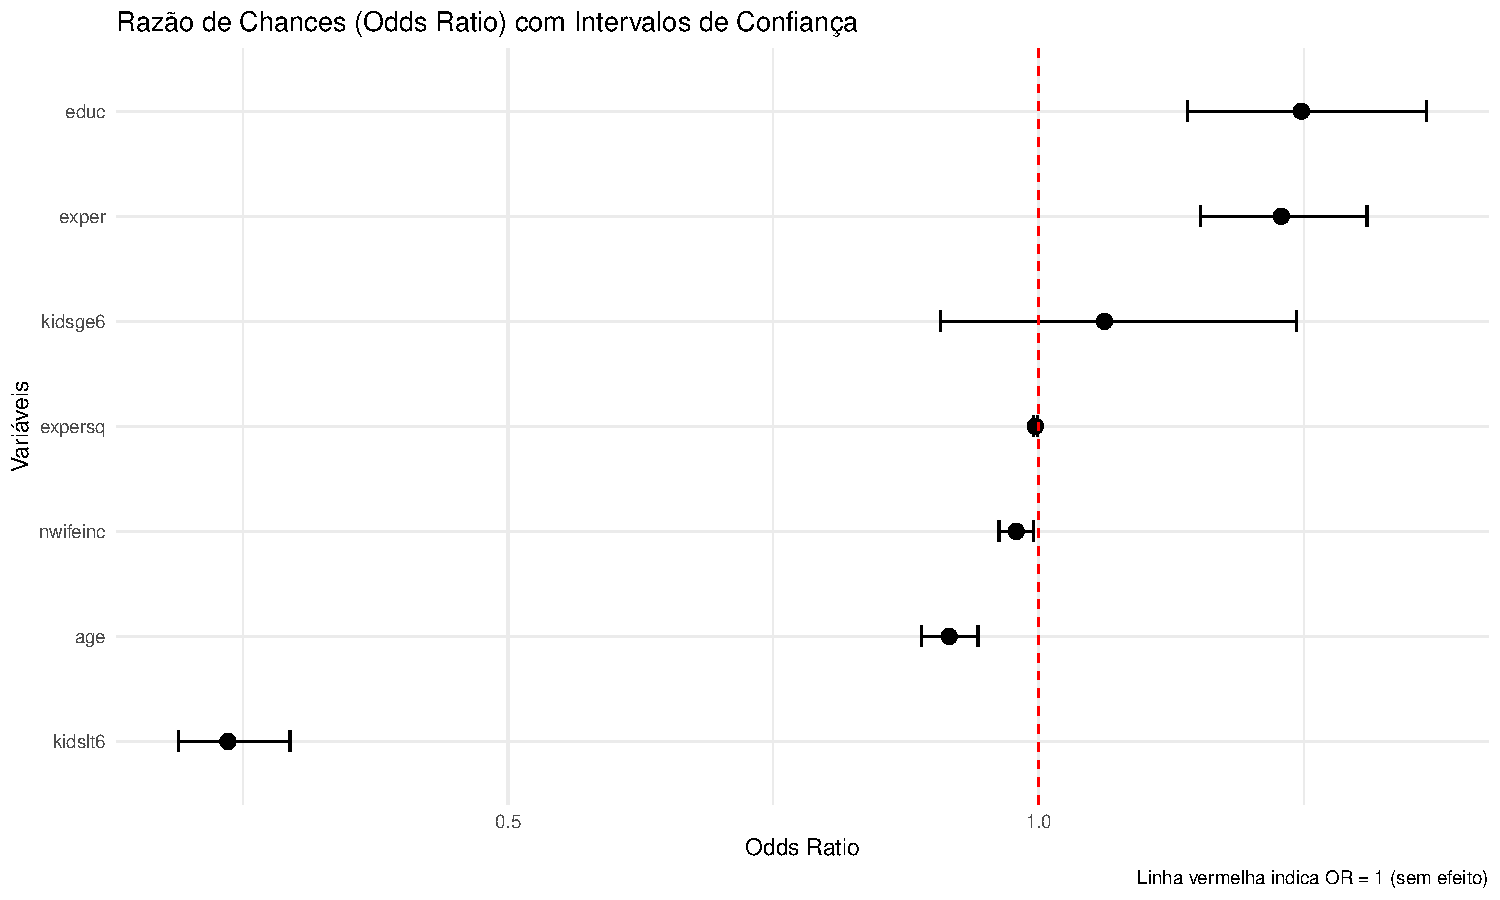
\includegraphics[keepaspectratio]{logit_probit_files/figure-pdf/odds-ratio-plot-1.pdf}}

\subsubsection{Interpretação da Razão de
Chances:}\label{interpretauxe7uxe3o-da-razuxe3o-de-chances-1}

\begin{itemize}
\tightlist
\item
  \textbf{OR = 1}: Não há diferença nas chances de ocorrência
\item
  \textbf{OR \textgreater{} 1}: Chances maiores de ocorrência do evento
\item
  \textbf{OR \textless{} 1}: Chances menores de ocorrência do evento
\end{itemize}

\subsection{Comparação Visual dos
Modelos}\label{comparauxe7uxe3o-visual-dos-modelos}

\begin{Shaded}
\begin{Highlighting}[]
\CommentTok{\# Comparação das funções de distribuição}
\NormalTok{x\_vals }\OtherTok{\textless{}{-}} \FunctionTok{seq}\NormalTok{(}\SpecialCharTok{{-}}\DecValTok{4}\NormalTok{, }\DecValTok{4}\NormalTok{, }\AttributeTok{length.out =} \DecValTok{100}\NormalTok{)}
\NormalTok{logistic\_vals }\OtherTok{\textless{}{-}} \DecValTok{1} \SpecialCharTok{/}\NormalTok{ (}\DecValTok{1} \SpecialCharTok{+} \FunctionTok{exp}\NormalTok{(}\SpecialCharTok{{-}}\NormalTok{x\_vals))}
\NormalTok{normal\_vals }\OtherTok{\textless{}{-}} \FunctionTok{pnorm}\NormalTok{(x\_vals)}

\NormalTok{comparison\_data }\OtherTok{\textless{}{-}} \FunctionTok{data.frame}\NormalTok{(}
  \AttributeTok{x =} \FunctionTok{rep}\NormalTok{(x\_vals, }\DecValTok{2}\NormalTok{),}
  \AttributeTok{y =} \FunctionTok{c}\NormalTok{(logistic\_vals, normal\_vals),}
  \AttributeTok{modelo =} \FunctionTok{rep}\NormalTok{(}\FunctionTok{c}\NormalTok{(}\StringTok{"Logística (Logit)"}\NormalTok{, }\StringTok{"Normal (Probit)"}\NormalTok{), }\AttributeTok{each =} \DecValTok{100}\NormalTok{)}
\NormalTok{)}

\NormalTok{p1 }\OtherTok{\textless{}{-}} \FunctionTok{ggplot}\NormalTok{(comparison\_data, }\FunctionTok{aes}\NormalTok{(}\AttributeTok{x =}\NormalTok{ x, }\AttributeTok{y =}\NormalTok{ y, }\AttributeTok{color =}\NormalTok{ modelo)) }\SpecialCharTok{+}
  \FunctionTok{geom\_line}\NormalTok{(}\AttributeTok{linewidth =} \FloatTok{1.2}\NormalTok{) }\SpecialCharTok{+}
  \FunctionTok{labs}\NormalTok{(}\AttributeTok{title =} \StringTok{"Comparação das Funções de Distribuição"}\NormalTok{,}
       \AttributeTok{x =} \StringTok{"X\textquotesingle{}β"}\NormalTok{,}
       \AttributeTok{y =} \StringTok{"P(Y=1|X)"}\NormalTok{,}
       \AttributeTok{color =} \StringTok{"Modelo"}\NormalTok{) }\SpecialCharTok{+}
  \FunctionTok{theme\_minimal}\NormalTok{()}

\CommentTok{\# Comparação das probabilidades preditas}
\NormalTok{p2 }\OtherTok{\textless{}{-}} \FunctionTok{ggplot}\NormalTok{(pred\_data, }\FunctionTok{aes}\NormalTok{(}\AttributeTok{x =}\NormalTok{ logit\_prob, }\AttributeTok{y =}\NormalTok{ probit\_prob)) }\SpecialCharTok{+}
  \FunctionTok{geom\_point}\NormalTok{(}\AttributeTok{alpha =} \FloatTok{0.6}\NormalTok{, }\FunctionTok{aes}\NormalTok{(}\AttributeTok{color =} \FunctionTok{factor}\NormalTok{(real))) }\SpecialCharTok{+}
  \FunctionTok{geom\_abline}\NormalTok{(}\AttributeTok{intercept =} \DecValTok{0}\NormalTok{, }\AttributeTok{slope =} \DecValTok{1}\NormalTok{, }\AttributeTok{linetype =} \StringTok{"dashed"}\NormalTok{) }\SpecialCharTok{+}
  \FunctionTok{labs}\NormalTok{(}\AttributeTok{title =} \StringTok{"Probabilidades Preditas: Logit vs Probit"}\NormalTok{,}
       \AttributeTok{x =} \StringTok{"Probabilidade Logit"}\NormalTok{,}
       \AttributeTok{y =} \StringTok{"Probabilidade Probit"}\NormalTok{,}
       \AttributeTok{color =} \StringTok{"Participação Real"}\NormalTok{) }\SpecialCharTok{+}
  \FunctionTok{theme\_minimal}\NormalTok{()}

\FunctionTok{grid.arrange}\NormalTok{(p1, p2, }\AttributeTok{ncol =} \DecValTok{2}\NormalTok{)}
\end{Highlighting}
\end{Shaded}

\pandocbounded{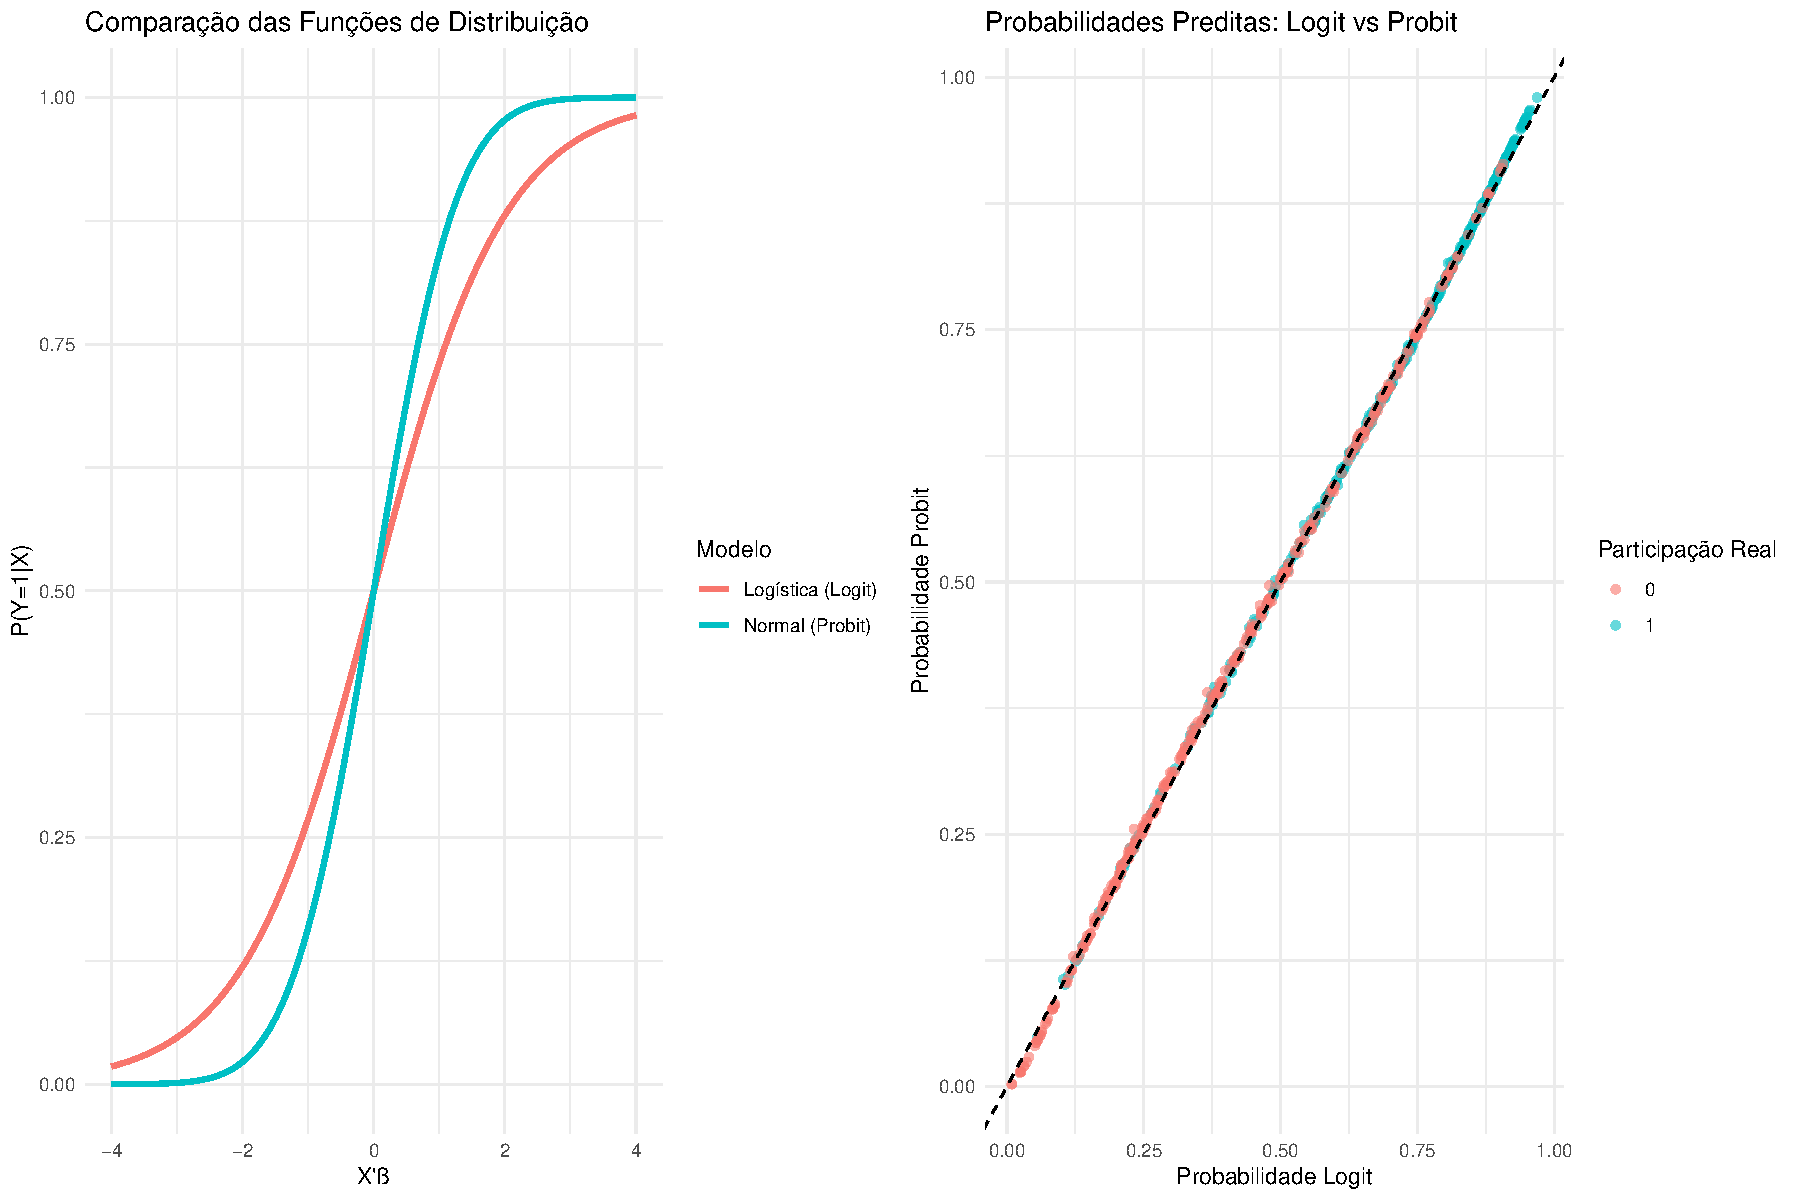
\includegraphics[keepaspectratio]{logit_probit_files/figure-pdf/model-comparison-1.pdf}}

\subsubsection{Análise Comparativa das
Funções}\label{anuxe1lise-comparativa-das-funuxe7uxf5es}

\textbf{Gráfico 1 - Funções de Distribuição:} - As funções
\textbf{Logística} e \textbf{Normal} são muito similares no intervalo
{[}-2, 2{]} - A função \textbf{Logística tem caudas mais pesadas} (decay
mais lento nos extremos) - Na prática, essa diferença tem
\textbf{impacto mínimo} nos resultados

\textbf{Gráfico 2 - Correlação das Probabilidades:} - \textbf{Correlação
quase perfeita} entre as probabilidades preditas pelos dois modelos -
Pontos próximos à \textbf{linha de 45°} indicam predições muito
similares - \textbf{Diferenças maiores} aparecem apenas nos extremos da
distribuição

\subsection{Resumo Comparativo dos
Modelos}\label{resumo-comparativo-dos-modelos}

\begin{Shaded}
\begin{Highlighting}[]
\CommentTok{\# Tabela resumo comparativa}
\NormalTok{summary\_comparison }\OtherTok{\textless{}{-}} \FunctionTok{data.frame}\NormalTok{(}
\NormalTok{  Critério }\OtherTok{=} \FunctionTok{c}\NormalTok{(}\StringTok{"AIC"}\NormalTok{, }\StringTok{"Log{-}Likelihood"}\NormalTok{, }\StringTok{"Pseudo{-}R²"}\NormalTok{, }\StringTok{"Acurácia (\%)"}\NormalTok{, }
               \StringTok{"Convergência"}\NormalTok{, }\StringTok{"Interpretação"}\NormalTok{, }\StringTok{"Uso Prático"}\NormalTok{),}
  \AttributeTok{Logit =} \FunctionTok{c}\NormalTok{(}\StringTok{"819.53"}\NormalTok{, }\StringTok{"{-}401.77"}\NormalTok{, }\StringTok{"0.2204"}\NormalTok{, }\StringTok{"73.57"}\NormalTok{, }\StringTok{"4 iterações"}\NormalTok{, }
            \StringTok{"Odds Ratios"}\NormalTok{, }\StringTok{"Mais comum"}\NormalTok{),}
  \AttributeTok{Probit =} \FunctionTok{c}\NormalTok{(}\StringTok{"818.60"}\NormalTok{, }\StringTok{"{-}401.30"}\NormalTok{, }\StringTok{"0.2206"}\NormalTok{, }\StringTok{"73.44"}\NormalTok{, }\StringTok{"4 iterações"}\NormalTok{, }
             \StringTok{"Efeitos marginais"}\NormalTok{, }\StringTok{"Base teórica"}\NormalTok{)}
\NormalTok{)}

\FunctionTok{kable}\NormalTok{(summary\_comparison, }\AttributeTok{caption =} \StringTok{"Resumo Comparativo: Logit vs Probit"}\NormalTok{)}
\end{Highlighting}
\end{Shaded}

\begin{longtable}[]{@{}lll@{}}
\caption{Resumo Comparativo: Logit vs Probit}\tabularnewline
\toprule\noalign{}
Critério & Logit & Probit \\
\midrule\noalign{}
\endfirsthead
\toprule\noalign{}
Critério & Logit & Probit \\
\midrule\noalign{}
\endhead
\bottomrule\noalign{}
\endlastfoot
AIC & 819.53 & 818.60 \\
Log-Likelihood & -401.77 & -401.30 \\
Pseudo-R² & 0.2204 & 0.2206 \\
Acurácia (\%) & 73.57 & 73.44 \\
Convergência & 4 iterações & 4 iterações \\
Interpretação & Odds Ratios & Efeitos marginais \\
Uso Prático & Mais comum & Base teórica \\
\end{longtable}

\subsection{Conclusões}\label{conclusuxf5es}

\subsubsection{Principais Achados}\label{principais-achados}

\begin{enumerate}
\def\labelenumi{\arabic{enumi}.}
\tightlist
\item
  \textbf{Ambos os modelos} apresentam resultados muito similares em
  termos de:

  \begin{itemize}
  \tightlist
  \item
    Significância dos coeficientes
  \item
    Direção dos efeitos
  \item
    Qualidade de ajuste (Pseudo-R² ≈ 0,22)
  \item
    Acurácia preditiva (\textasciitilde73,5\%)
  \end{itemize}
\item
  \textbf{Variáveis mais importantes}:

  \begin{itemize}
  \tightlist
  \item
    \textbf{kidslt6}: forte efeito negativo (presença de filhos pequenos
    reduz participação em 35 p.p.)
  \item
    \textbf{educ}: efeito positivo forte (cada ano aumenta participação
    em 5,4 p.p.)
  \item
    \textbf{exper}: efeito positivo com retornos decrescentes
  \item
    \textbf{age}: efeito negativo (idade avançada reduz participação)
  \item
    \textbf{nwifeinc}: efeito negativo pequeno (maior renda familiar
    reduz necessidade de trabalhar)
  \end{itemize}
\item
  \textbf{Variável não significativa}:

  \begin{itemize}
  \tightlist
  \item
    \textbf{kidsge6}: filhos mais velhos não afetam significativamente a
    decisão de trabalhar
  \end{itemize}
\end{enumerate}

\subsubsection{Escolha entre Modelos}\label{escolha-entre-modelos}

\begin{Shaded}
\begin{Highlighting}[]
\CommentTok{\# Critérios de decisão}
\NormalTok{decision\_table }\OtherTok{\textless{}{-}} \FunctionTok{data.frame}\NormalTok{(}
\NormalTok{  Situação }\OtherTok{=} \FunctionTok{c}\NormalTok{(}\StringTok{"Melhor ajuste estatístico"}\NormalTok{, }\StringTok{"Interpretação via chances"}\NormalTok{, }
               \StringTok{"Base teórica sólida"}\NormalTok{, }\StringTok{"Facilidade computacional"}\NormalTok{, }
               \StringTok{"Tradição na literatura"}\NormalTok{),}
  \StringTok{\textasciigrave{}}\AttributeTok{Modelo Preferido}\StringTok{\textasciigrave{}} \OtherTok{=} \FunctionTok{c}\NormalTok{(}\StringTok{"Probit (AIC ligeiramente menor)"}\NormalTok{, }\StringTok{"Logit (Odds Ratios)"}\NormalTok{, }
                         \StringTok{"Probit (distribuição normal)"}\NormalTok{, }\StringTok{"Logit (convergência mais rápida)"}\NormalTok{, }
                         \StringTok{"Logit (mais utilizado)"}\NormalTok{)}
\NormalTok{)}

\FunctionTok{kable}\NormalTok{(decision\_table, }\AttributeTok{caption =} \StringTok{"Critérios para Escolha entre Logit e Probit"}\NormalTok{)}
\end{Highlighting}
\end{Shaded}

\begin{longtable}[]{@{}ll@{}}
\caption{Critérios para Escolha entre Logit e Probit}\tabularnewline
\toprule\noalign{}
Situação & Modelo.Preferido \\
\midrule\noalign{}
\endfirsthead
\toprule\noalign{}
Situação & Modelo.Preferido \\
\midrule\noalign{}
\endhead
\bottomrule\noalign{}
\endlastfoot
Melhor ajuste estatístico & Probit (AIC ligeiramente menor) \\
Interpretação via chances & Logit (Odds Ratios) \\
Base teórica sólida & Probit (distribuição normal) \\
Facilidade computacional & Logit (convergência mais rápida) \\
Tradição na literatura & Logit (mais utilizado) \\
\end{longtable}

\subsubsection{Recomendações
Práticas}\label{recomendauxe7uxf5es-pruxe1ticas}

\begin{enumerate}
\def\labelenumi{\arabic{enumi}.}
\item
  \textbf{Para esta aplicação específica}: Ambos os modelos são
  adequados, com \textbf{ligeira vantagem para o Probit} em termos de
  ajuste (AIC menor)
\item
  \textbf{Para interpretação}: O \textbf{modelo Logit} oferece vantagem
  pela facilidade de interpretação via \textbf{odds ratios}
\item
  \textbf{Para pesquisa acadêmica}: A escolha pode depender da
  \textbf{tradição da área} ou \textbf{preferências teóricas}
\item
  \textbf{Para predição}: Ambos apresentam \textbf{performance
  equivalente} (diferença de acurácia \textless{} 0,2\%)
\end{enumerate}

\subsubsection{Implicações para Política
Pública}\label{implicauxe7uxf5es-para-poluxedtica-puxfablica}

Os resultados sugerem pontos importantes para políticas de participação
feminina no mercado de trabalho:

\begin{enumerate}
\def\labelenumi{\arabic{enumi}.}
\item
  \textbf{Creches e cuidado infantil}: O forte efeito negativo de
  \texttt{kidslt6} sugere que políticas de apoio ao cuidado de crianças
  pequenas poderiam aumentar significativamente a participação feminina
\item
  \textbf{Educação}: O efeito positivo robusto da educação reforça a
  importância de investimentos em educação feminina
\item
  \textbf{Experiência profissional}: Programas de capacitação e
  experiência profissional têm potencial de impacto positivo
\item
  \textbf{Idade}: Políticas direcionadas a mulheres mais jovens podem
  ser mais efetivas
\end{enumerate}

\subsubsection{Limitações do Estudo}\label{limitauxe7uxf5es-do-estudo}

\begin{enumerate}
\def\labelenumi{\arabic{enumi}.}
\tightlist
\item
  \textbf{Dados de 1975}: Os padrões podem ter mudado significativamente
  nas últimas décadas
\item
  \textbf{Amostra específica}: Resultados limitados a mulheres casadas
  nos EUA
\item
  \textbf{Variáveis omitidas}: Outros fatores importantes podem não
  estar incluídos (atitudes sociais, disponibilidade de emprego, etc.)
\item
  \textbf{Causalidade}: As relações estimadas são associações, não
  necessariamente causais
\end{enumerate}

\subsubsection{Próximos Passos}\label{pruxf3ximos-passos}

Para futuras pesquisas, sugere-se: 1. \textbf{Atualização dos dados}
para períodos mais recentes 2. \textbf{Inclusão de variáveis adicionais}
(atitudes, normas sociais) 3. \textbf{Análise por subgrupos} (idade,
educação, região) 4. \textbf{Modelos de efeitos fixos} para controlar
heterogeneidade não observada




\end{document}
